%%% \documentclass[%
%%% reprint,
%%% twocolumn,
%%% %superscriptaddress,
%%% %groupedaddress,
%%% %unsortedaddress,
%%% %runinaddress,
%%% %frontmatterverbose,
%%% % preprint,
%%% showpacs,
%%% showkeys,
%%% preprintnumbers,
%%% %nofootinbib,
%%% %nobibnotes,
%%% %bibnotes,
%%% amsmath,amssymb,
%%% aps,
%%% prl,
%%% % pra,
%%% % prb,
%%% % rmp,
%%% %prstab,
%%% %prstper,
%%% longbibliography,
%%% %floatfix,
%%% %lengthcheck,%
%%% ]{revtex4-1}
%%%
%%% %\usepackage{cdmtcs-pdf}
%%%
%%% \usepackage[dvipsnames]{xcolor}
%%%
%%% \usepackage{mathptmx}% http://ctan.org/pkg/mathptmx
%%%
%%% \usepackage{amssymb,amsthm,amsmath}
%%%
%%% \usepackage{tikz}
%%% \usetikzlibrary{calc,decorations.pathreplacing,decorations.markings,positioning,shapes}
%%%
%%% \usepackage[breaklinks=true,colorlinks=true,anchorcolor=blue,citecolor=blue,filecolor=blue,menucolor=blue,pagecolor=blue,urlcolor=blue,linkcolor=blue]{hyperref}
%%% \usepackage{graphicx}% Include figure files
%%% \usepackage{url}
%%%
%%%
%%% \begin{document}
%%%
%%% \title{Classical predictions for intertwined quantum observables are contingent and thus inconclusive}
%%% %\title{Unconditional classical predictions of intertwined quantum observables are contingent}
%%% %\title{The empirical trouble with classical analyses of quantum clouds}
%%%
%%%
%%% \author{Karl Svozil}
%%% \email{svozil@tuwien.ac.at}
%%% \homepage{http://tph.tuwien.ac.at/~svozil}
%%%
%%% \affiliation{Institute for Theoretical Physics,
%%% Vienna University of Technology,
%%% Wiedner Hauptstrasse 8-10/136,
%%% 1040 Vienna, Austria}
%%%
%%%
%%%
%%% \date{\today}
%%%
%%% \begin{abstract}
%%% Classical evaluations of configurations of intertwined quantum contexts induce relations, such as true-implies-false, true-implies-true~\cite{2018-minimalYIYS}, but also nonseparability among the input and output terminals. When combined, these exploitable configurations (also known as gadgets) deliver the strongest form of classical value indefiniteness. However, the choice of the respective configuration among all such collections, and thus the relation of its terminals, remains arbitrary and cannot be motivated by some superselection principle inherent to quantum or classical physics.
%%% \end{abstract}
%%%
%%% %\keywords{Quantum mechanics, Gleason theorem, Kochen--Specker theorem, Born rule, gadget graphs}
%%%
%%% \maketitle


\PassOptionsToPackage{dvipsnames}{xcolor}
\documentclass[quantumrep,article,accept,oneauthor,pdftex]{Definitions/mdpi}


%%%%%%%%%%%%%%%%%%%%%%%%%%%%%%%%%%%%%%%%%%%%%%%%%%%%%%%%%%%%%%%%%%%%%%%%%%%%%%%%%%%%%%%%%%%%%%%%%%%%%%%%%%%%%%%%%%%%%%%%%%%%%%%%%%%%%%%%%%%%%%%%
\usepackage{graphicx}% Include figure files

\usepackage{amssymb}

\usepackage{tikz}
\usetikzlibrary{calc,decorations.pathreplacing,decorations.markings,positioning,shapes}

\newcommand{\ruledtabular}{\hline \hline}

%%%%%%%%%%%%%%%%%%%%%%%%%%%%%%%%%%%%%%%%%%%%%%%%%%%%%%%%%%%%%%%%%%%%%%%%%%%%%%%%%%%%%%%%%%%%%%%%%%%%%%%%%%%%%%%%%%%%%%%%%%%%%%%%%%%%%%%%%%%%%%%%



\firstpage{1}
\makeatletter
\setcounter{page}{\@firstpage}
\makeatother
\pubvolume{xx}
\issuenum{1}
\articlenumber{5}
\pubyear{2020}
\copyrightyear{2020}
\history{Received: date; Accepted: date; Published: date}
\updates{yes} % If there is an update available, un-comment this line

%% MDPI internal command: uncomment if new journal that already uses continuous page numbers
%\continuouspages{yes}

%------------------------------------------------------------------
% The following line should be uncommented if the LaTeX file is uploaded to arXiv.org
%\pdfoutput=1

%=================================================================
% Add packages and commands here. The following packages are loaded in our class file: fontenc, calc, indentfirst, fancyhdr, graphicx, lastpage, ifthen, lineno, float, amsmath, setspace, enumitem, mathpazo, booktabs, titlesec, etoolbox, amsthm, hyphenat, natbib, hyperref, footmisc, geometry, caption, url, mdframed, tabto, soul, multirow, microtype, tikz
\setitemize{parsep=6pt,itemsep=0pt,leftmargin=*,labelsep=5.5mm}
\setenumerate{parsep=6pt,itemsep=0pt,leftmargin=*,labelsep=5.5mm}
\setlist[description]{itemsep=0mm}
%=================================================================
%% Please use the following mathematics environments: Theorem, Lemma, Corollary, Proposition, Characterization, Property, Problem, Example, ExamplesandDefinitions, Hypothesis, Remark, Definition, Notation, Assumption
%% For proofs, please use the proof environment (the amsthm package is loaded by the MDPI class).

%=================================================================
% Full title of the paper (Capitalized)
\Title{Classical Predictions for Intertwined Quantum Observables are Contingent and Thus Inconclusive}%Attention AE/ME. The following layout issues have not been checked by the English Editing Department and must be carefully verified by the AE/Layout Department: All callout issues, bold usage of callouts, and references to callouts in the text. Correct callout usage in figures. Figure and Table layout issues. Footnote formatting and Glossaries have not been checked. En dash usage for negative values, en dash usage to indicate relationships, en dash usage to indicate bonds (especially in chemistry). The English Editing Department is not responsible for correct italic usage for genes, proteins and technical terminology. This responsibility belongs to the authors. The following are also not checked: spacing between numbers and units of measurement, ratios, en dashes for ranges, date and time formats, punctuation in equation lines, and less than/more than spacing (< >). Finally, capitalization and layout of titles/headings must be properly checked as well as ensuring 'Eq.' and 'Fig.' are properly spelled out, as these are layout issues.
%\thanks{This is a largely revised and extended version of a paper which has been published somewhat hidden in Section~12.9 of my recent book on (A)Causality~\cite{svozil-pac}.}

% Author Orchid ID: enter ID or remove command
\newcommand{\orcidauthorA}{0000-0001-6554-2802} % Add \orcidA{} behind the author's name

% Authors, for the paper (add full first names)
\Author{Karl Svozil \orcidA{}}

% Authors, for metadata in PDF
\AuthorNames{Karl Svozil}

% Affiliations / Addresses (Add [1] after \address if there is only one affiliation.)
\address[1]{%
Institute for Theoretical Physics, Vienna University of Technology, Wiedner Hauptstrasse 8-10/136, A-1040~Vienna, Austria; svozil@tuwien.ac.at}

% Contact information of the corresponding author
%\corres{Correspondence: e-mail@e-mail.com; Tel.: (optional; include country code; if there are multiple corresponding authors, add author initials) +xx-xxxx-xxx-xxxx (F.L.)}

% Current address and/or shared authorship
%\firstnote{Current address: Affiliation 3}
%\secondnote{These authors contributed equally to this work.}
% The commands \thirdnote{} till \eighthnote{} are available for further notes

%\simplesumm{} % Simple summary

%\conference{} % An extended version of a conference paper

% Abstract (Do not insert blank lines, i.e. \\)
\abstract{Classical evaluations of configurations of intertwined quantum contexts induce relations, such as true-implies-false and true-implies-true, but also nonseparability among the input and output terminals. When combined, these exploitable configurations (also known as gadgets) deliver the strongest form of classical value indefiniteness. However, the choice of the respective configuration among all such collections, and thus the relation of its terminals, remains arbitrary and cannot be motivated by some superselection principle inherent to quantum or classical physics.} % reference citation not allow show in abstract
% Keywords
\keyword{quantum mechanics; Gleason theorem; Kochen--Specker theorem; Born rule; gadget graphs}

% The fields PACS, MSC, and JEL may be left empty or commented out if not applicable
\PACS{03.65.Ca; 02.50.-r; 02.10.-v; 03.65.Aa; 03.67.Ac; 03.65.Ud}
%\MSC{}
%\JEL{}

%%%%%%%%%%%%%%%%%%%%%%%%%%%%%%%%%%%%%%%%%%
% Only for the journal Diversity
%\LSID{\url{http://}}

%%%%%%%%%%%%%%%%%%%%%%%%%%%%%%%%%%%%%%%%%%
% Only for the journal Applied Sciences:
%\featuredapplication{Authors are encouraged to provide a concise description of the specific application or a potential application of the work. This section is not mandatory.}
%%%%%%%%%%%%%%%%%%%%%%%%%%%%%%%%%%%%%%%%%%

%%%%%%%%%%%%%%%%%%%%%%%%%%%%%%%%%%%%%%%%%%
% Only for the journal Data:
%\dataset{DOI number or link to the deposited data set in cases where the data set is published or set to be published separately. If the data set is submitted and will be published as a supplement to this paper in the journal Data, this field will be filled by the editors of the journal. In this case, please make sure to submit the data set as a supplement when entering your manuscript into our manuscript editorial system.}

%\datasetlicense{license under which the data set is made available (CC0, CC-BY, CC-BY-SA, CC-BY-NC, etc.)}

%%%%%%%%%%%%%%%%%%%%%%%%%%%%%%%%%%%%%%%%%%
% Only for the journal Toxins
%\keycontribution{The breakthroughs or highlights of the manuscript. Authors can write one or two sentences to describe the most important part of the paper.}

%\setcounter{secnumdepth}{4}
%%%%%%%%%%%%%%%%%%%%%%%%%%%%%%%%%%%%%%%%%%
\begin{document}



\section{Quantum Clouds as Collections of Intertwined Contexts and Their Classical Doubles}

Quantum logic, as conceived of by von Neumann~\cite{v-neumann-49,v-neumann-55} and Birkhoff~\cite{birkhoff-36},
is about the formal/theoretical universe of potential empirical observable propositions,
as well as the algebraic relations and operations among them.
Every single one of these observables is considered operational ``subject to the experimenter's grace'',
as its actual measurement reflects the experimenter's (subjective) choice to indeed measure one of these
potential observables, {versus} its (often continuity of) complementary ones
(this choice is mostly supposed to be {``ex machina''}; that is, outside of the reach of quantum theory,
and not subject to nesting~\cite{everett,wigner:mb,everett-1956}).
Thereby, all the other, then counterfactual, observables remain in a ``dormant/hypothetical'' realm,
an idealist~\cite{berkeley,stace} ``limbo'' of sorts.

Even explorations allowing logical operations exclusively among simultaneously commeasurable observables~\cite{Kochen2,Kochen3}
and permitting partial value definiteness~\cite{2012-incomput-proofsCJ,2015-AnalyticKS}
(in the recursion-theoretic sense of Kleene~\cite{Kleene1936})
rely upon, and are thus valid relative to, such collections of counterfactuals.
Thereby, the predictions/forecasts
derived not for a single such collection of observables---here sometimes referred to as cloud or gadget---but for (finite) selections from the multitude of conceivable (finite) collections of observables
may be inconsistent.


One way to conceptualize the (nonclassical) performance of quantized systems is in terms of (black) boxes
with input and output terminals as interfaces~\cite{2018-minimalYIYS}.
Like zero-knowledge proofs~\cite{Quisquater1990} (a~topic the late Specker became interested in),
they are supposed to certify that they act ``truly quantum mechanically''
while at the same time not allowing any inspection (e.g., duplication or opening)
other than their performance at the input-output
terminals.
Fulfillment/certification is usually obtained by the exhibition of certain features or signals usually not encountered by classical devices, among them complementarity
and classical value indefiniteness (mostly pronounced as contextuality).
For a great variety of such criteria, see Table~\ref{2018-c-table1-conc-rel-info},
as well as the references cited therein, later.

However, the signals obtained from these boxes are far from plain.
Indeed, in what follows, we shall argue that,
depending on which hypothetical configurations of (necessarily complementary) ``intrinsic'' observables are
considered, any individual outcome can {ad hoc} be classically (re)interpreted as an indication of nonclassicality.
Yet, the same outcome could also be in full conformity with a~classical interpretation.
A combination of such classical models allows any statistical prediction at the terminals.
Moreover,
there does not seem to exist any convincing reason to choose one
of such configurations over another, thus giving rise to either contradictory or arbitrary {ad hoc} signal analysis.

Already, Specker~\cite{Specker-60} contemplated about generalized exotic behaviors even beyond quantum boxes,
whereby his criteria for ``weirdness'' were inspired by scholastic counterfactuals
(also known as {Infuturabilien}).
The benign outcome of his fable was only made possible by the unmarried daughter's determined, alas futile, attempt to open
the ``wrong''---according to her father's strategy---box; at which point, he gave in, and marriage ensued.
Quantum boxes and, as will be later argued, quantum clouds are not dissimilar: because
of complementarity
and classical value indefiniteness (also known as contextuality),
complete knowledge of the situation is impossible by any known physical means.
An immediate idealistic~\cite{berkeley,stace,Goldschmidt2017-idealism}
objection to the use of counterfactuals could
be that the presupposition of the sort of omni-realism required for a classical analysis of quantum boxes
cannot be operational~\cite{bridgman} and supported by quantum mechanics.
Indeed, the partial algebra approach of Kochen and Specker~\cite{Kochen2,Kochen3,Kochen1}
disallows operations among complementary observables
whilst making heavy use of intertwined collections of complementary maximal operators (also known as contexts).


However, even classical models based on set representable partition logics~\cite{svozil-2001-eua}
such as Moore's initial state identification problem~\cite{e-f-moore}
%for what would later become (irreversible) finite automata theory in computer science,
and also Wright's generalized urn model~\cite{wright:pent,wright}
mimic quantum complementarity to a certain degree---indeed,
formally up to quantum logics with separable sets of two-valued states~(\cite{Kochen1}, Theorem~0, p.~67).
Thereby, nonseparability of quantum observables with respect to the set
of two-valued states (interpretable as classical truth assignments)
serves as a strict criterion for nonclassicality
and also as a criterion against realizations by set-theoretical representable partition logics,
even if such two-valued states exist.



In what follows, we shall further exploit counterfactual
configurations of contexts that are intertwined (this terminology is borrowed from Gleason~\cite{Gleason})
in one or more common observable(s).
Such counterfactual configurations of contexts will be called {clouds}.

Graph theoretically~(\cite{Godsil-Newman-2008}, Appendix),
a context can be associated with a complete graph (also known as a clique).
Its vertices are identified with the elements of the context.
Adjacency is characterized by comeasurable exclusivity.
Clouds are represented by collections of complete graphs (also known as  cliques
 or contexts) intertwining at the respective vertices,
thereby leaving the edges unchanged.


In quantum mechanics, contexts are identified with orthonormal bases,
or equivalently with the maximal operators~(\cite{halmos-vs}, \S~84, Theorem~1, p.~171),
which can be (nonuniquely) formed by nondegenerate sums containing all the one-dimensional orthogonal projection operators
associated with those respective bases.
Elementary propositions are formalized by vectors of these bases of $d$-dimensional Hilbert space,
or by the orthogonal projection operators associated with such vectors~\cite{birkhoff-36}.
Graph theoretically, the vertices are represented by the basis vectors,
and adjacency stands for the orthogonality of these vectors;
that is, the edges represent the (pairwise) orthogonality
relations between the vectors (vertices)
(each vertex must be connected to all the other $d-1$ vertices in the respective context by an edge).
Thereby, the graph representing a cloud
has a faithful orthogonal representation~\cite{lovasz-89,Portillo-2015}
in terms of the elements of the bases representing the respective contexts.
The inverse problem of finding some faithful orthogonal representation of a given graph is still open.
A necessary condition for the existence of intertwines is that the dimensionality of the
vector space is higher than two because in fewer dimensions than three, contexts are either identical or disjoint.

Orthogonality hypergraphs~\cite{greechie:71} are compact representations of clouds
that reveal their structural constituents by signifying contexts/cliques/bases:
every complete graph $K_d$ is replaced by a {single smooth curve} (usually a straight line)
containing distinguished points that represent the vertices.
Thereby, the $d(d - 1)/2$ edges of any such complete graph $K_d$ are replaced with a single smooth curve.
All the vertices ``within'' this smooth curve represent the mutually orthogonal vectors forming a $d$-dimensional basis.


Clouds may have various model realizations and representations: a particular cloud may have:
\begin{itemize}[leftmargin=21pt,labelsep=7pt]
\item[(i)] a quantum mechanical realization in terms of intertwining orthonormal bases, as mentioned~earlier;
\item[(ii)] a pseudo-classical realization in terms of partition logic, which in turn have automaton logic or generalized urn models;
\item[(iii)] a classical realization if there is only a single context involved;
\item[(iv)] none of the above (such as a tightly interlinked ``triangle'' configuration of three contexts with two vertices per context).
\end{itemize}

Suffice it to say that (i) does not imply (ii), and vice versa.
Case (iii) can be interpreted as
a subalgebra of all the other groups enumerated, as the cases (i) and (ii) are pastings of contexts or (Boolean) blocks~\cite{nav:91}.

\section{Enforcing Classical Two-Valued States}

The commonly used method for exploring nonclassicality is to consider
configurations of type (i) with a quantum realization, upon which a classical interpretation, if it exists,
is ``enforced'' in terms of uniform classical truth and falsity allocations of the associated propositions.
Such value assignments
can be formalized by two-valued states $s \in \{0,1\}$ or (classical truth) value assignments,
which are additive and add up to one whenever the propositions are exclusive and within a single context.

The physical intuition behind this formalization is the observation that any $d$-dimensional context or maximal observable
can be interpreted as an array of detectors after a $d$-port beam splitter~\cite{rzbb}.
In~an ideal experiment, only one detector clicks (associated with the proposition that the system is in the respective state),
whereas all the other $d-1$ detectors remain silent.


Such uniform classical interpretations are supposed to be context-independent;
that is, the value on intertwining observables, which are common to two or more contexts, is independent
of the context.
Besides the context-independence of truth assignments at the intertwining observables, various variants of such measures assume conditions of increasing strength:
\begin{itemize}[leftmargin=21pt,labelsep=7pt]
\item[(I)] The ``measures'' or value assignments employed in so-called ``contextuality inequalities''
merely assume that every proposition is either true or false,
regardless of the other propositions in that context, which are simultaneously measurable~\cite{cabello:210401}.
This allows all possible $2^d$ possibilities of value assignments in a $d$-dimensional context with $d$ vertices,
thereby vastly expanding the multitude of possible value assignments.
With this expansion, all Kochen--Specker sets trivially allow value~assignments.
\item[(II)] The prevalent assumption of two-valued states or value assignments, also used by Kochen and Specker~\cite{Kochen1}, as well as Pitowsky~\cite{pitowsky:218},
is that only a {single} one of the $d$ vertices within a~$d$-dimensional context
is true, and all the others are false; therefore, any isolated $d$-dimensional context can have only $d$ such standard two-valued value assignments.
\item[(III)] \textls[20]{An even more restricted rule of value assignment abandons uniform definiteness
and} supposes~\cite{2012-incomput-proofsCJ,PhysRevA.89.032109,2015-AnalyticKS} that,
if all $d-1$ but one vertex in a $d$-dimensional context are false, the~remaining one is true,
and if one vertex within a $d$-dimensional context is true, all remaining $d-1$ vertices are false.
These latter value assignments allow for {partial} functions, which can be undefined.
\end{itemize}

Type (III) implies
Type (II), which in turn implies Type (I) value assignments.

A set $S$ of two-valued states on a graph $G$ is~\cite{svozil-tkadlec,tkadlec-96}:
\begin{itemize}[leftmargin=21pt,labelsep=7pt]
\item[(u)] {unital}, if for every $x\in G$, there is a two-valued state $s\in S$
such that $s(x) = 1$;
\item[(s)] {separating}, if for every distinct pair of vertices $x,y\in G$
with $x\neq y$, there is an $s\in S$ such that $s (x) \neq s (y)$;
\item[(f)] {full}, if for every nonadjacent pair of vertices $x,y\in G$,
there is an $s \in S$ such that $s (x) = s (y) = 1$.
\end{itemize} % please confirm the Numbering if is right

A full set of
two-valued states is separating,
and a separating set of
two-valued states is unital.
As will be detailed later TIFS%define if appropriate
/10-gadgets have a nonfull set, so two-valued states in the sense of~(f).
Nonseparability in the sense of~(s) indicates nonclassicality.
Nonunitality in the sense of~(u) discredits the classical predictions of quantum clouds
even to a greater degree, probably only challenged by a complete absence of two-valued states.


\section{Chromatic Separability}

As already discussed by Kochen and Specker~(\cite{Kochen1}, Theorem~0),
nonseparability of (at least one) a pair of nonadjacent vertices
with respect to the set of two-valued states
(interpretable as classical truth assignments) of a graph
is arguably the most important signature of nonclassicality.
It may be true even if there is an ``abundance'' of two-valued states.
Nonseparability can also be expressed in terms of graph coloring.

 A proper (vertex)
coloring~(\cite{Godsil-Newman-2008}, Appendix) of a graph is a function $c$ from the vertex set to a~finite
set of ``colors'' (the positive integers will do) such that,
whenever $x$ and $y$ are adjacent vertices,
$c(x) \neq c(y)$.
The chromatic number of a graph is the least positive integer $t$ such
that the graph has a~coloring with $t$ colors.


A two-valued state on a (hyper)graph composed/pasted from contexts/cliques,
all having an~identical
number of vertices/clique numbers $d$, can be obtained by ``projecting/reducing'' colors
if the chromatic number of that graph equals $d$.
In this case, in order to obtain a two-valued state,
take any proper (vertex) coloring $c$ with $d$ colors
and map $d-1$ colors into (the ``new color'') zero and one~color into (the ``new color'') one.
Just as the graph coloring $c$ itself, such mappings need not to be unique.

Note that the chromatic number of a complete graph must be equal to the clique number
because Type~(II)~{and}~(III) two-valued states require that every context/clique
must have exactly one vertex with value assignment~one (and~zero for all the other vertices)
(one might conjecture that the set of two-valued states
induces graph colorings, in much the same way as it induces a partition logic~\cite{svozil-2001-eua}).
At the same time, the clique number renders a bound from below on the chromatic number.
Thus, if the chromatic number of a graph exceeds the clique number,
no such two-valued states exist; the ``phenomenological consequence'' is that, for at least one context/clique,
the color projection/reduction is constant---namely zero---on all vertices of that context/clique.



A coloring is {chromatically separating} two nonadjacent distinct vertices $x$ and $y$ in the vertex set of a graph
if there exists a proper vertex coloring such that $c(x) \neq c(y)$.
A set of colorings of a particular graph is said to be {separating}
if, for any pair of distinct vertices, it contains at least one coloring, which separates those vertices.
The {separable chromatic number} of a graph is the least positive integer $t$ such
that the graph has a separating set of colorings with at most $t$ colors.

If the separable chromatic number is higher than the chromatic number of a given graph,
then~there exist nonadjacent vertices that cannot be ``resolved''
by any proper graph coloring, or, for~that matter, by any derived
projected/reduced two-valued state.
As a consequence, the graph has no set-theoretic realization as a partition logic,
although its chromatic number is the clique number,
and~there still may exist an abundance of proper colorings and two-valued states~(\cite{Kochen1}, $\Gamma_3$, p.~70).

It would be interesting to translate (non)unitality and (non)fullness into (sets of) graph coloring.
For reasons of brevity, we shall not discuss this here.



\section{Formation of Gadgets as Useful Subgraphs for the Construction of Clouds}

The commonly used method seeks cloud configurations with ``exotic'' classical interpretations.
Again, exoticism may express itself in various forms or types.
One way is in terms of violations on bounds on classical {conditions of possible experience}~(\cite{Boole-62}, p.~229),
such as Bell-type inequalities derivable from taking all (Type~(II),
and Type~(I) for inequalities using only the assumption of noncontextuality~\cite{cabello:210401}) value assignments,
forming a correlation polytope by encoding those states into vertices, and solving the hull problem
thereof~\cite{froissart-81,cirelson,pitowsky-86,pitowsky,pitowsky-89a,Pit-91,Pit-94,2000-poly}.
Another, stronger~\cite{svozil-2011-enough} form of nonclassicality is the nonexistence
of any such classical interpretation in terms of a Type~(II) valued
assignments~\cite{Gleason,Specker-60,Zierler1975,Kochen1,pitowsky:218};
or at least their nonseparability~(\cite{Kochen1}, Theorem~0, p.~67).

The explicit construction of such exotic classical interpretations
often proceeds by the (successive) application of exploitable subconfigurations of contexts; in graph theoretical terms, {gadgets}~\cite{tutte_1954,SZABO2009436,Ramanathan-18} defined as ``useful subgraphs''.
Thereby, gadgets are formed from constituent lower order gadgets of ever-increasing size and functional performance
(see also~(\cite{svozil-2016-pu-book}, Chapter~12)):
\begin{enumerate}

\item Zeroth order gadget: a single context (also known as clique/block/Boolean (sub)algebra/maximal observable/orthonormal basis).
This can be perceived as the most elementary form of a~true-implies-false (TIFS/10)~\cite{2018-minimalYIYS}/01-(maybe better 10)-gadget~\cite{svozil-2006-omni,Ramanathan-18}
configuration, because a~truth/value one assignment of one of the vertices implies falsity/value zero assignments of all the~others;

\item First order ``firefly'' gadget: two contexts connected in a single intertwining vertex;

\item Second order gadget: two first order firefly gadgets connected in a single intertwining vertex;

\item Third order house/pentagon/pentagram gadget: one firefly and one second order gadget connected in two intertwining vertices to form a cyclic orthogonality hypergraph;

\item Fourth order 10-gadget: e.g., a Specker bug~\cite{2018-minimalYIYS} consisting of two pentagon gadgets connected by an entire context;
as well as extensions thereof to arbitrary angles for the terminal (``extreme'') points~\cite{2015-AnalyticKS,Ramanathan-18};

\item Fifth order true-implies-true (TITS)~\cite{2018-minimalYIYS}/11-gadget~\cite{svozil-2006-omni}: e.g., Kochen and Specker's $\Gamma_1$~\cite{Kochen1}, consisting of one 10-gadget and one firefly gadget,
connected at the respective terminal points (cf.~Figure~6).
% please confirm if it is invalid mention
%\item 6th order gadget: e.g., Kochen and Specker's $\Gamma_3$~\cite{Kochen1}, consisting of a combo of two TITS/11-gadgets, connected by their common firefly gadgets;
%
%\item 7th order construction: consisting of one 10- and one 11-gadget with identical terminal points serving as constructions of Pitowsky's
%principle of indeterminacy~\cite{2015-AnalyticKS,svozil-2018-whycontexts};
%
%\item 8th order construction: the concatenation of (10- and) 11-gadgets pasted/stitched together to form a graph used for proofs of the Kochen--Specker theorem;
%e.g., Kochen and Specker's $\Gamma_2$~\cite{Kochen1}.
\end{enumerate}

That is, gadgets are subconfigurations of clouds. Clouds can be interpreted as gadgets for the composition of bigger clouds.

For the sake of arguing for an idealistic~\cite{berkeley,stace,Goldschmidt2017-idealism} and against a realistic usage of quantum clouds,
configurations of intertwined contexts with two fixed propositions
as ``start'' and ``end'' points ${\bf a}$~and ${\bf b}$ will be studied;
as well as methods for constructing such configurations with particular {relational} properties.
Whenever there is no preferred, less so unique, path connecting ${\bf a}$ and ${\bf b}$, all such connections should be treated on an equal basis.
We shall call any such collection of counterfactual connections ``{clouds} connecting ${\bf a}$ and ${\bf b}$'',
denoted by $C({\bf a},{\bf b})$, and depict it with a cloud shape symbol,
as drawn in Figure~\ref{2018-c-fcloud} (this can in principle be generalized to more than two terminal points).
\begin{figure}[H]
\begin{center}
\begin{tikzpicture} [scale=0.25]

\tikzstyle{every path}=[line width=2pt]

\newdimen\ms
\ms=0.1cm

\tikzstyle{s1}=[color=red,rectangle,inner sep=3.5]
\tikzstyle{c3}=[circle,inner sep={\ms/8},minimum size=5*\ms]
\tikzstyle{c2}=[circle,inner sep={\ms/8},minimum size=3*\ms]
\tikzstyle{c1}=[circle,inner sep={\ms/8},minimum size=2*\ms]

% Radius of regular polygons
\newdimen\R
\R=14.5cm % outer circle

%\r= { \R * sqrt(3) } % inner circle
%\newdimen\r
%\r= {\R * sqrt(3)/2}  % inner circle

%\newdimen\K
%\K=3cm

% Define positions of all observables
\path
 ({180 + 0 * 360 /2}:\R  ) coordinate(1)
 ({180 + 1 * 360 /2}:\R ) coordinate(2)
;

% draw contexts

%\draw [draw=violet!30] (0,0) circle[radius=\R ] node[above right] { };

\draw [color=orange] (1) -- (2);

\node[cloud, cloud puffs=15.7, cloud ignores aspect, minimum width=4.5cm, minimum height=3cm, align=center, draw] (cloud) [color=black,fill=red!5] at (0cm, 0cm) {\Large{\color{black}\vspace{1cm} intertwined contexts \vspace{1cm} }};


%
%%
%% draw atoms
%%
%

\draw (1) coordinate[c3,fill=black]; %
\draw (1) coordinate[c2,fill=black!20,label=180:\colorbox{white}{\Large ${\bf a}$}]; %

\draw (2) coordinate[c3,fill=black]; %
\draw (2) coordinate[c2,fill=black!20,label=right:\colorbox{white}{\Large ${\bf b}$}]; %
%
\end{tikzpicture}
\end{center}
\caption{
\label{2018-c-fcloud}
A collection of possible connections of counterfactuals organized in intertwining contexts and joining ${\bf a}$ and ${\bf b}$, depicted as a cloud
$C({\bf a},{\bf b})$.}
\end{figure}




Thereby, as the endpoints ${\bf a}$ and ${\bf b}$ remain fixed, one can ask what kind of (classical) {relational information} can
be inferred from such two-point quantum clouds.
%(Generalizations to three- or higher-point quantum clouds will not be studied here.)
As it turns out, for fixed ${\bf a}$ and ${\bf b}$, quantum clouds can be found that realize a wide variety
of conceivable relational properties between ${\bf a}$ and ${\bf b}$.
Table~\ref{2018-c-table1-conc-rel-info} enumerates these relations.
%%% \begingroup
%%% \squeezetable
\begin{table}[H]
\centering \small
\caption{Some (incomplete) history of the relational properties realizable by two-point quantum clouds.}
\label{2018-c-table1-conc-rel-info}
%%% \begin{ruledtabular}
\scalebox{0.95}[0.95]{
\begin{tabular}{lll}
\toprule
\textbf{If A is True} & \textbf{Anecdotal, Historic} & \textbf{Reference to Utility} \\
\textbf{Classical Value Assignments} & \textbf{Quantum Realization} & \textbf{or Relational Properties}\\
\midrule
imply ${\bf b}$ is independent (arbitrary) & firefly logic $L_{12}$~(\cite{cohen}, pp.~21,~22)& \\
imply ${\bf b}$ false (TIFS%define if appropriate
/10) & Specker bug logic~(\cite{Kochen2}, Figure~1, p.~182) & (\cite{stairs83}, pp.~588--589), \cite{Yu-2012,2018-minimalYIYS}\\
imply ${\bf b}$ true (TITS%define if appropriate
) & extended Specker bug logic & (\cite{Kochen1}, $\Gamma_1$, p.~68), \\
&&(\cite{clifton-93}, Sects.~II, III, Figure~1), \\
&&(\cite{Belinfante-73}, Figure~C.l. p.~67), \\
&&(\cite{Pitowsky-1982-subs}, p.~394), \cite{Hardy-92,Hardy-93,hardy-97}, \\
&&\cite{Cabello-1995-ppks,cabello-96,cabello-97-nhvp,Badziag-2011,Cabello-2013-HP,Cabello-2013-Hardylike,2018-minimalYIYS}\\
iff ${\bf b}$ true (nonseparability) & combo of intertwined Specker bugs & (\cite{Kochen1}, $\Gamma_3$, p.~70)\\
imply value indefiniteness of ${\bf b}$ & depending on Type (II), (III) assignments & \cite{pitowsky:218,2015-AnalyticKS}\\
\bottomrule
\end{tabular}
}
%%% \end{ruledtabular}
\end{table}
%%% \endgroup

\section{Quantum Clouds Enforcing Particular Features When Interpreted Classically}

For quantum mechanics, ${\bf a}$ and ${\bf b}$ can be
formalized by the two one-dimensional projection operators
$\textsf{\textbf{E}}_{\bf a} =\vert {\bf a} \rangle \langle {\bf a}\vert$ and
$\textsf{\textbf{E}}_{\bf b} =\vert {\bf b} \rangle \langle {\bf b}\vert$, respectively.
For the sake of demonstration, we shall study configurations in which
$\vert {\bf a} \rangle = \begin{pmatrix}1,0,0\end{pmatrix}$
and
$\vert {\bf b} \rangle = \begin{pmatrix} \frac{1}{\sqrt{2}},\frac{1}{2},\frac{1}{2} \end{pmatrix}$,
that is the quantum prediction yields a~probability $\vert \langle {\bf b} \vert {\bf a} \rangle \vert^2 = \frac{1}{2}$
of finding
the quantum in a state $\vert {\bf b} \rangle$ if it has been prepared in a state $\vert {\bf a}\rangle$.
This~configuration can be extended to endpoints with (noncollinear and nonorthogonal) arbitrary relative location
by the techniques introduced in~\cite{2015-AnalyticKS,Ramanathan-18}.

\begin{enumerate}[leftmargin=2.3em,labelsep=4mm]
\item[(a)]
A quantum cloud configuration for which classical value assignments allow
${\bf b}$ to be either true or false if ${\bf a}$ is true
is the firefly configuration~(\cite{cohen}, pp.~21--22), depicted in Figure~\ref{2018-c-f-firefly},
with five classical value assignments of Type (II)~\cite{dvur-pul-svo}.
\begin{figure}[H]
\begin{center}
\begin{tikzpicture} [scale=0.20]

\newdimen\ms
\ms=0.05cm

\tikzstyle{every path}=[line width=1.5pt]

\tikzstyle{s1}=[color=red,rectangle,inner sep=3]
\tikzstyle{c4}=[circle,inner sep={\ms/8},minimum size=4*\ms]
\tikzstyle{c3}=[circle,inner sep={\ms/8},minimum size=3*\ms]
\tikzstyle{c2}=[circle,inner sep={\ms/8},minimum size=2*\ms]
\tikzstyle{c1}=[circle,inner sep={\ms/8},minimum size=1*\ms]

% Radius of regular polygons
\newdimen\R
\R=6cm % outer circle

%\r= { \R * sqrt(3) } % inner circle
%\newdimen\r
%\r= {\R * sqrt(3)/2}  % inner circle

%\newdimen\K
%\K=3cm

% Define positions of all observables
\path
 (0,6 ) coordinate(1)
 (3,3 ) coordinate(2)
 (6,0 ) coordinate(3)
 (9,3) coordinate(4)
 (12,6 ) coordinate(5)
;

% draw contexts

\draw [color=orange] (1) -- (2) -- (3);
\draw [color=blue] (3) -- (4) -- (5);


%
%%
%% draw atoms
%%
%
\draw (1) coordinate[s1,draw=black,fill=red,label={above left: \footnotesize $\vert {\bf a} \rangle = \begin{pmatrix}1,0,0\end{pmatrix}$}]; %
%
\draw (2) coordinate[c3,draw=green,fill=green,label={left: \footnotesize $\frac{1}{\sqrt{2}}\begin{pmatrix}0,1,1\end{pmatrix}$}]; %
%
\draw (3) coordinate[c3,draw=green,fill=green,label={below: \footnotesize $\frac{1}{\sqrt{2}}\begin{pmatrix}0,1,-1\end{pmatrix}$}]; %
%\draw (3) coordinate[c2,fill=orange]; %
%
\draw (4) coordinate[c3,draw=black,fill=white,label={right: \footnotesize $\begin{pmatrix} -\frac{1}{\sqrt{2}},\frac{1}{2},\frac{1}{2}\end{pmatrix}$}]; %
%
\draw (5) coordinate[c4,draw=black,fill=white,label={above right: \footnotesize $\vert {\bf b} \rangle = \begin{pmatrix} \frac{1}{\sqrt{2}},\frac{1}{2},\frac{1}{2} \end{pmatrix}$}]; %
%
%

\end{tikzpicture}
\end{center}
\caption{
\label{2018-c-f-firefly}
Orthogonality hypergraph of a cloud consisting of a
firefly logic $L_{12}$ connecting ${\bf a}$ and ${\bf b}$, such that, for Type (II) value assignments, ${\bf a}$~true-implies-${\bf b}$~whatever (quantum 50:50).
Truth is encoded by a filled red square, classical falsity by a filled green circle, and arbitrary truth values by circles
(Type (III) value assignments are partial and thus undefined).
$L_{12}$ consists of five~vertices in just two~intertwined blocks allowing
a separating set of five~two-valued states and therefore a set representable by partition~logics.}
\end{figure}


\item[(b)]
Already, Kochen and Specker utilized quantum clouds enforcing classical ${\bf a}$~true-implies-${\bf b}$~false predictions
and their compositions in the construction of a configuration that does not allow a uniform truth assignment (of Type (II)).
Stairs~(\cite{stairs83}, pp.~588--589) has pointed out that the Specker bug~(\cite{Kochen2}, Figure~1, p.~182)
is a quantum cloud configuration that classically enforces ${\bf a}$~true-implies-${\bf b}$~false:
if a quantum system is prepared in such a way that ${\bf a}$ is true---that is, if~it is in the state $\textsf{\textbf{E}}_{\bf a}$--and measured along $\textsf{\textbf{E}}_{\bf b}$, and
$\vert {\bf a} \rangle$ and
$\vert {\bf b} \rangle$
are not orthogonal or collinear, then any observation of ${\bf b}$ given ${\bf a}$ amounts to a probabilistic proof of nonclassicality:
because although quantum probabilities do not vanish, classical value assignments predict that ${\bf b}$ never occurs.
Minimal quantum cloud configurations for classical ${\bf a}$~true-implies-${\bf b}$~false,
as well as ${\bf a}$~true-implies-${\bf b}$~true value assignments (of Type (II)) can be found in~\cite{2018-minimalYIYS}.

As Cabello has pointed out~\cite{cabello-1994,Cabello-1996-diss}, the original Specker bug configuration cannot go beyond
the quantum prediction probability threshold $\vert \langle {\bf b} \vert {\bf a} \rangle \vert^2 = 3^{-2}$
because the angle between ${\bf a}$ and ${\bf b}$ cannot be smaller than
$\arccos {\frac{1}{3}} \approx 1.23096$ radians ($71.5^\circ$).
A configuration~(\cite{svozil-2018-whycontexts}, Figure~5a) allowing Type (III) TIFS truth assignments
with ``maximally unbiased''
quantum prediction probability $\vert \langle {\bf b} \vert {\bf a} \rangle \vert^2 = \frac{1}{2}$
is a sublogic of a quantum logic
whose realization was enumerated in \cite{2015-AnalyticKS}, Table.~1, p.~102201-7.
This is depicted in Figure~\ref{2018-c-f-TIFS}.
A proof of Theorem~2 in~\cite{Ramanathan-18} contains an explicit parametrization of a single
TIFS/10~cloud allowing the full range of angles $0 < \angle {\bf a},{\bf b} < \pi$.
\begin{figure}[H]
\newif\iflabel \labelfalse
\begin{center}
\begin{tikzpicture} [scale=0.25, rotate=117]

  \tikzstyle{every path}=[line width=1.5pt]
  \tikzstyle{c1}=[color=green,circle,inner sep=2.0]
  \tikzstyle{s1}=[color=red,rectangle,inner sep=2.5]
  \tikzstyle{l1}=[draw=none,circle,minimum size=4]

  % Define positions of all observables

%\draw [color=orange] (4,0) coordinate[c1,fill,label=0:{\color{black}\footnotesize $\vert {\bf b} \rangle = \begin{pmatrix} \frac{1}{\sqrt{2}},\frac{1}{2},\frac{1}{2} \end{pmatrix}$}] (b) -- (13,0) coordinate[c1,fill,label=270:{\iflabel \tiny $P_2$\fi}] (2) -- (22,0) coordinate[s1,fill,label=315:{\iflabel \tiny $P_3$\fi}] (3);
\draw [color=orange] (4,0) coordinate[c1,draw=black,fill,label=0:{\color{black}\footnotesize $\vert {\bf b} \rangle$}] (b) -- (13,0) coordinate[c1,fill,label=270:{\iflabel \tiny $P_2$\fi}] (2) -- (22,0) coordinate[s1,fill,label=315:{\iflabel \tiny $P_3$\fi}] (3);
\draw [color=blue, ] (3) -- (26,12) coordinate[c1,fill,pos=0.8,label=0:{\iflabel \tiny $P_{21}$\fi}] (21) coordinate[c1,fill,label=0:{\iflabel \tiny $P_{23}$\fi}] (23);
\draw [color=white] (23) -- (22,18.5) coordinate[c1,fill,pos=0.4,color=white,label=0:{\iflabel \tiny $P_{29}$\fi}] (29) coordinate[c1,fill,label=45:{\iflabel \tiny $P_5$\fi}] (5);
%\draw [color=magenta,] (5)-- (13,18.5)coordinate[s1,fill,label=180:{\color{black}\footnotesize $\vert {\bf a} \rangle = \begin{pmatrix}1,0,0\end{pmatrix}$}] (a) -- (4,18.5) coordinate[c1,fill,label=135:{\iflabel \tiny $P_4$\fi}] (4);
\draw [color=magenta,] (5)-- (13,18.5)coordinate[s1,draw=black,fill,label=180:{\color{black}\footnotesize $\vert {\bf a} \rangle$}] (a) -- (4,18.5) coordinate[c1,fill,label=135:{\iflabel \tiny $P_4$\fi}] (4);
\draw [color=CadetBlue, ] (4) -- (0,12) coordinate[c1,fill,pos=0.6,label=180:{\iflabel \tiny $P_{10}$\fi}] (10) coordinate[s1,fill,label=180:{\iflabel \tiny $P_7$\fi}] (7);
\draw [color=brown, ](7) -- (b)  coordinate[c1,fill,pos=0.2,label=180:{\iflabel \tiny $P_6$\fi}] (6);

  \draw [color=gray] (a) -- (2) coordinate[c1,fill,pos=0.5,label=315:{\iflabel \tiny $P_1$\fi}] (1);

  \draw [color=violet] (5) -- (22,6) coordinate[s1,fill,pos=0.4,label=0:{\iflabel \tiny $P_{11}$\fi}] (11) coordinate[c1,fill,label=0:{\iflabel \tiny $P_9$\fi}] (9);

\draw [color=Apricot] (9) -- (b) coordinate[s1,fill,pos=0.3,label=280:{\iflabel \tiny $P_8$\fi}] (8);

\draw [color=TealBlue] (4) -- (4,6) coordinate[s1,fill,pos=0.4,label=180:{\iflabel \tiny $P_{28}$\fi}] (28) coordinate[c1,fill,label=180:{\iflabel \tiny $P_{22}$\fi}] (22);
\draw [color=YellowGreen] (22) -- (3) coordinate[c1,fill,pos=0.2,label=260:{\iflabel \tiny $P_{19}$\fi}] (19);

  \coordinate (25) at ([xshift=-4cm]1);
  \coordinate (27) at ([xshift=4cm]1);

\draw [color=MidnightBlue] (22) -- (25) coordinate[c1,fill,pos=0.5,label=115:{\iflabel \tiny $P_{24}$\fi}] (24) coordinate[s1,fill,label=270:{\iflabel \tiny $P_{25}$\fi}] (25);
\draw [color=Mulberry] (25) -- (9) coordinate[c1,fill,pos=0.8,label=90:{\iflabel \tiny $P_{35}$\fi}] (35);

\draw [color=BrickRed] (7) -- (27) coordinate[c1,fill,pos=0.5,label=90:{\iflabel \tiny $P_{34}$\fi}] (34) coordinate[c1,fill,label=90:{\iflabel \tiny $P_{27}$\fi}] (27);
\draw [color=Emerald] (27) -- (23) coordinate[s1,fill,pos=0.25,label=270:{\iflabel \tiny $P_{26}$\fi}] (26);

\draw [color=BlueGreen] (10) -- (15.5,17.5) coordinate[c1,fill,pos=0.5,label=90:{\iflabel \tiny $P_{12}$\fi}] (12) coordinate[s1,fill,label=15:{\iflabel \tiny $P_{13}$\fi}] (13);
%\draw [color=Tan] (13) -- (29) coordinate[c1,fill,pos=0.4,label=90:{\iflabel \tiny $P_{31}$\fi}] (31);

\draw [color=RawSienna] (28) -- (10.5,15) coordinate[c1,fill,pos=0.5,label=90:{\iflabel \tiny $P_{30}$\fi}] (30) coordinate[c1,fill,label=90:{\iflabel \tiny $P_{15}$\fi}] (15);
\draw [color=SpringGreen] (15) -- (11) coordinate[c1,fill,pos=0.6,label=90:{\iflabel \tiny $P_{14}$\fi}] (14);

\draw [color=Salmon] (15) -- (1) coordinate[s1,fill,pos=0.2,label=15:{\iflabel \tiny $P_{17}$\fi}] (17);
\draw [color=Fuchsia] (1)-- (13) coordinate[c1,fill,draw=black,pos=0.3,label=90:{\color{black}\footnotesize $\vert {16} \rangle$}] (16);

\draw [color=CornflowerBlue] (19) -- (16) coordinate[s1,fill,pos=0.3,label=180:{\iflabel \tiny $P_{18}$\fi}] (18);
\draw [color=pink] (16) -- (8) coordinate[c1,fill,pos=0.7,label=180:{\iflabel \tiny $P_{32}$\fi}] (32);

\draw [color=PineGreen] (6) -- (17) coordinate[c1,fill,pos=0.7,label=90:{\iflabel \tiny $P_{33}$\fi}] (33);
\draw [color=DarkOrchid] (17) -- (21) coordinate[c1,fill,pos=0.4,label=90:{\iflabel \tiny $P_{20}$\fi}] (20);

\draw [color=black] (25) -- (1) -- (27);

%\coordinate (ContextLabel) at ([shift=({-2cm,-3mm})]1);
%\draw (ContextLabel) coordinate[l1,label=90:{\iflabel \tiny $C_{26}$\fi}];

\end{tikzpicture}
\end{center}
\caption{\label{2018-c-f-TIFS}
Orthogonality hypergraph of a nonfull/TIFS/10~cloud even for Type (III) value assignments.
A faithful orthogonal realization was enumerated in~\cite{2015-AnalyticKS}, Table.~1, p.~102201-7.
It consists of 38~vertices in 24~intertwined blocks,
endowed with a nonseparating set of 13~two-valued states and therefore is not set representable by partition logics.
The state depicted is the only one allowing ${\bf a}$ to be one.
Moreover, this cloud has no unital set of two-valued states, as for all of them, the vertex
represented by the vector
$
\vert {16} \rangle
=
\frac{1}{\sqrt{10}}
\left(
2\sqrt{2},1,-1
\right)
$ and
drawn as a solid black circle (and the associated
observable) needs to be zero at all classical instantiations.
}
\end{figure}

%$$$$$$$$$$$$$$$$$$$$$$$$$$$$$$$$$$$$$$$$$$$$$$

\item[(c)]
Clifton (note added in the proof to Stairs~(\cite{stairs83}, pp.~588--589))
presented a ${\bf a}$~true-implies-${\bf b}$~true (TITS) cloud~(\cite{clifton-93,Johansen-1994,Vermaas-1994}, Sects.~II, III, Figure~1)
inspired by Bell~(\cite{Belinfante-73}, Figure~C.l. p.~67) (cf. also Pitowsky~(\cite{Pitowsky-1982-subs}, p.~394)),
as well as by the Specker bug logic~(\cite{clifton-93}, Sects.~IV, Figure~2).
Hardy~\cite{Hardy-92,Hardy-93,hardy-97},
as well as Cabello, among others~\cite{cabello-1994,Cabello-1996-diss,cabello-96,cabello-97-nhvp,Badziag-2011,Cabello-2013-HP,Cabello-2013-Hardylike,Ramanathan-18},
utilized similar scenarios for the demonstration of nonclassicality~(\cite{svozil-pac}, Chapter~14).
Figure~\ref{2018-c-f-TITS} depicts an 11-gadget~(\cite{svozil-2018-whycontexts}, Figure~5b) with identical endpoints as the 10-gadget
discussed earlier and depicted in Figure~\ref{2018-c-f-TIFS}.

\item[(d)]
Various parallel and serial compositions of 10- and 11-gadgets serve as a ``gadget toolbox'' to obtain clouds, which, if they are interpreted classically,
exhibit other interesting relational properties.
For instance, the parallel composition (pasting) of two quantum clouds of the 10-gadget type:
one 10-gadget classically demanding ${\bf a}$~true-implies-${\bf b}$~false
and the other 10-gadget classically demanding ${\bf b}$~true-implies-${\bf a}$~false, results in a quantum cloud that has two observables ${\bf a}$ and ${\bf b}$,
which are classically always ``opposite'': if one is true, the other one is false, and {vice versa}.

\item[(e)]
The parallel composition (pasting) of two quantum clouds of the TITS type, with one TITS, classically demanding ${\bf a}$~true-implies-${\bf b}$~true
and the other TITS classically demanding ${\bf b}$~true-implies-${\bf a}$~true, results in a quantum cloud that has two observables ${\bf a}$ and ${\bf b}$,
which are classically nonseparable, which is a sufficient criterion for nonclassicality~(\cite{Kochen1}, Theorem~0, p.~67).
As pointed out by Portillo~\cite{Portillo-2018-pc}, this is equivalent to ${\bf a}$ is true if and only if ${\bf b}$ is true (TIFFTS%define if appropriate
).
Figure~\ref{2018-c-f-TIFFTS} depicts a historic example of such a construction.
The serial composition of suitable TITS
of the form ${\bf a}_1$~true-implies-${\bf a}_2 \cdots {\bf a}_{i-1}$~true-implies-${\bf a_i}$~true
eventually yields two or more vectors ${\bf a}_1$ and ${\bf a_i}$ that are mutually orthogonal; a technique employed by Kochen and Specker
for the construction of a quantum cloud admitting no Type (II) truth assignment~(\cite{Kochen1}, $\Gamma_2$, p.~69).
\begin{figure}[H]
\newif\iflabel
\labelfalse
\begin{center}
\begin{tikzpicture} [scale=0.25, rotate=117]

  \tikzstyle{every path}=[line width=1.5pt]
  \tikzstyle{c1}=[color=green,circle,inner sep=2.0]
  \tikzstyle{s1}=[color=red,rectangle,inner sep=2.5]
  \tikzstyle{l1}=[draw=none,circle,minimum size=4]

  % Define positions of all observables


\draw [color=orange] (4,0) coordinate[s1,draw=black,fill,label=0:{\color{black}\footnotesize $\vert {\bf b}\rangle$}] (b) -- (13,0) coordinate[c1,fill,label=270:{\iflabel \tiny $P_2$\fi}] (2) -- (22,0) coordinate[c1,fill,label=315:{\iflabel \tiny $P_3$\fi}] (3);
\draw [color=blue, ] (3) -- (26,12) coordinate[c1,fill,pos=0.8,label=0:{\iflabel \tiny $P_{21}$\fi}] (21) coordinate[s1,fill,label=0:{\iflabel \tiny $P_{23}$\fi}] (23);
\draw [color=green] (23) -- (22,18.5) coordinate[c1,fill,pos=0.4,label=0:{\iflabel \tiny $P_{29}$\fi}] (29) coordinate[c1,fill,label=45:{\iflabel \tiny $P_5$\fi}] (5);
\draw [color=magenta,] (5)-- (13,18.5)coordinate[s1,draw=black,fill,label=180:{\color{black}\footnotesize $\vert {\bf a}\rangle$}] (a) -- (4,18.5) coordinate[c1,fill,label=135:{\iflabel \tiny $P_4$\fi}] (4);
\draw [color=white] (4) -- (0,12) coordinate[c1,color=white,fill,pos=0.6,label=180:{\iflabel \tiny $P_{10}$\fi}] (10) coordinate[c1,fill,label=180:{\iflabel \tiny $P_7$\fi}] (7);
\draw [color=brown, ] (7) -- (b) coordinate[c1,fill,pos=0.2,label=180:{\iflabel \tiny $P_6$\fi}] (6);

 \draw [color=gray] (a) -- (2) coordinate[c1,fill,pos=0.5,label=315:{\iflabel \tiny $P_1$\fi}] (1);

 \draw [color=violet] (5) -- (22,6) coordinate[s1,fill,pos=0.4,label=0:{\iflabel \tiny $P_{11}$\fi}] (11) coordinate[c1,fill,label=0:{\iflabel \tiny $P_9$\fi}] (9);

\draw [color=Apricot] (9) -- (b) coordinate[c1,fill,pos=0.3,label=280:{\iflabel \tiny $P_8$\fi}] (8);

\draw [color=TealBlue] (4) -- (4,6) coordinate[s1,fill,pos=0.4,label=180:{\iflabel \tiny $P_{28}$\fi}] (28) coordinate[c1,fill,label=180:{\iflabel \tiny $P_{22}$\fi}] (22);
\draw [color=YellowGreen] (22) -- (3) coordinate[s1,fill,pos=0.2,label=260:{\iflabel \tiny $P_{19}$\fi}] (19);

 \coordinate (25) at ([xshift=-4cm]1);
 \coordinate (27) at ([xshift=4cm]1);

\draw [color=MidnightBlue] (22) -- (25) coordinate[c1,fill,pos=0.5,label=115:{\iflabel \tiny $P_{24}$\fi}] (24) coordinate[s1,fill,label=270:{\iflabel \tiny $P_{25}$\fi}] (25);
\draw [color=Mulberry] (25) -- (9) coordinate[c1,fill,pos=0.8,label=90:{\iflabel \tiny $P_{35}$\fi}] (35);

%\draw [color=BrickRed] (7) -- (27) coordinate[c1,fill,pos=0.5,label=90:{\iflabel \tiny $P_{34}$\fi}] (34) coordinate[c1,fill,label=90:{\iflabel \tiny $P_{27}$\fi}] (27);
\draw [color=BrickRed] (7) -- (27) coordinate[s1,fill,pos=0.5,label=90:{\iflabel \tiny $P_{34}$\fi}] (34) coordinate[c1,fill,label=90:{\iflabel \tiny $P_{27}$\fi}] (27);
\draw [color=Emerald] (27) -- (23) coordinate[c1,fill,pos=0.25,label=270:{\iflabel \tiny $P_{26}$\fi}] (26);

\draw [color=white] (10) -- (15.5,17.5) coordinate[c1,color=white,fill,pos=0.5,label=90:{\iflabel \tiny $P_{12}$\fi}] (12) coordinate[s1,fill,label=15:{\iflabel \tiny $P_{13}$\fi}] (13);
\draw [color=Tan] (13) -- (29) coordinate[c1,fill,pos=0.4,label=90:{\iflabel \tiny $P_{31}$\fi}] (31);

\draw [color=RawSienna] (28) -- (10.5,15) coordinate[c1,fill,pos=0.5,label=90:{\iflabel \tiny $P_{30}$\fi}] (30) coordinate[c1,fill,label=90:{\iflabel \tiny $P_{15}$\fi}] (15);
\draw [color=SpringGreen] (15) -- (11) coordinate[c1,fill,pos=0.6,label=90:{\iflabel \tiny $P_{14}$\fi}] (14);

\draw [color=Salmon] (15) -- (1) coordinate[s1,fill,pos=0.2,label=15:{\iflabel \tiny $P_{17}$\fi}] (17);
\draw [color=Fuchsia] (1)-- (13) coordinate[c1,fill,draw=black,pos=0.3,label=90:{\color{black}\footnotesize $\vert {16} \rangle$}] (16);

\draw [color=CornflowerBlue] (19) -- (16) coordinate[c1,fill,pos=0.3,label=180:{\iflabel \tiny $P_{18}$\fi}] (18);
\draw [color=pink] (16) -- (8) coordinate[s1,fill,pos=0.7,label=180:{\iflabel \tiny $P_{32}$\fi}] (32);

\draw [color=PineGreen] (6) -- (17) coordinate[c1,fill,pos=0.7,label=90:{\iflabel \tiny $P_{33}$\fi}] (33);
\draw [color=DarkOrchid] (17) -- (21) coordinate[c1,fill,pos=0.4,label=90:{\iflabel \tiny $P_{20}$\fi}] (20);

\draw [color=black] (25) -- (1) -- (27);

 \coordinate (ContextLabel) at ([shift=({-2cm,-3mm})]1);
 \draw (ContextLabel) coordinate[l1,label=90:{\iflabel \tiny $C_{26}$\fi}];

 \end{tikzpicture}
\end{center}
\caption{
\label{2018-c-f-TITS}
Orthogonality hypergraph of a TITS/11 cloud even for Type (III) value assignments.
A~faithful orthogonal realization was enumerated in~\cite{2015-AnalyticKS}, Table.~1, p.~102201-7.
It consists of 38~vertices in 24~intertwined blocks,
endowed with a nonseparating set of 13~two-valued states and therefore is not set representable by partition logics.
The state depicted is the only one allowing ${\bf a}$ to be one.
Moreover, this cloud has no unital set of two-valued states, as for all of them, the vertex
represented by the vector $\vert {16} \rangle = \frac{1}{\sqrt{10}}\left( 2\sqrt{2},1,-1 \right)$ and
drawn as a solid black circle (and the associated
observable) needs to be zero at all classical instantiations.
}
\end{figure}

\begin{figure}[H]
\begin{center}
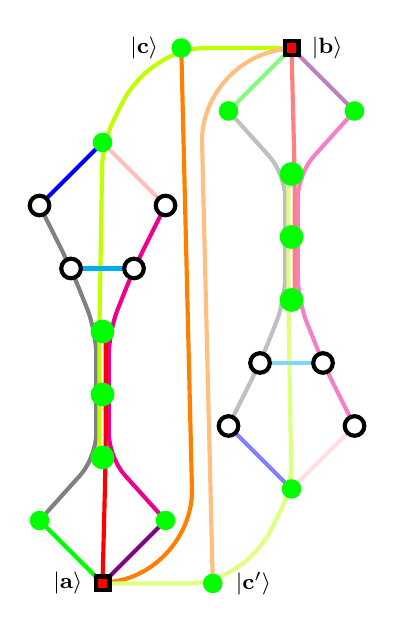
\begin{tikzpicture} [scale=0.8, rotate= 0]

% Epsilon
\newdimen\E
\E=0.05 cm

\tikzstyle{every path}=[line width=1.5pt]


% Epsilon
\newdimen\ms
\ms=0.15 cm
%\tikzstyle{c4}=[circle,inner sep={\ms/8},minimum size=4*\ms]
%\tikzstyle{c3}=[circle,inner sep={\ms/8},minimum size=3*\ms]
%\tikzstyle{c2}=[circle,inner sep={\ms/8},minimum size=2*\ms]
%\tikzstyle{c1}=[circle,inner sep={\ms/8},minimum size=1.1*\ms]

  \tikzstyle{c1}=[color=green,circle,inner sep=2.5]
  \tikzstyle{s1}=[color=red,rectangle,inner sep=2.5]


% Define positions of all observables
\path
 (1,0)   coordinate(1)
 (0,1)   coordinate(2)
 (2,1)   coordinate(3)
 ({1 cm-2*\E},2) coordinate(4)
 ({1 cm-1*\E},2) coordinate(5)
 ({1 cm+1*\E},2) coordinate(6)
 ({1 cm+2*\E},2) coordinate(7)
 ({1 cm-2*\E},3) coordinate(8)
 ({1 cm-1*\E},3) coordinate(9)
 ({1 cm+1*\E},3) coordinate(10)
 ({1 cm+2*\E},3) coordinate(11)
 ({1 cm-2*\E},4) coordinate(12)
 ({1 cm-1*\E},4) coordinate(13)
 ({1 cm+1*\E},4) coordinate(14)
 ({1 cm+2*\E},4) coordinate(15)
 (0.5,5)   coordinate(16)
 (1.5,5)   coordinate(17)
 (0,6)   coordinate(18)
 (2,6)   coordinate(19)
 (1,7)   coordinate(20)
 (2.25,8.5)  coordinate(21)
 (4,8.5)   coordinate(22)
 (2.45,0.25)  coordinate(23) %auxiliary
 (1.5,8)  coordinate(24) %auxiliary
 (1,2)  coordinate(25) %auxiliary
 (1,3)  coordinate(26) %auxiliary
 (1,4)  coordinate(27) %auxiliary

 (3,0)+(1,8.5)   coordinate(101)
 (3,0)+(0,7.5)   coordinate(102)
 (3,0)+(2,7.5)   coordinate(103)
 (3,0)+({1 cm-2*\E},6.5) coordinate(104)
 (3,0)+({1 cm-1*\E},6.5) coordinate(105)
 (3,0)+({1 cm+1*\E},6.5) coordinate(106)
 (3,0)+({1 cm+2*\E},6.5) coordinate(107)
 (3,0)+({1 cm-2*\E},5.5) coordinate(108)
 (3,0)+({1 cm-1*\E},5.5) coordinate(109)
 (3,0)+({1 cm+1*\E},5.5) coordinate(110)
 (3,0)+({1 cm+2*\E},5.5) coordinate(111)
 (3,0)+({1 cm-2*\E},4.5) coordinate(112)
 (3,0)+({1 cm-1*\E},4.5) coordinate(113)
 (3,0)+({1 cm+1*\E},4.5) coordinate(114)
 (3,0)+({1 cm+2*\E},4.5) coordinate(115)
 (3,0)+(0.5,3.5)   coordinate(116)
 (3,0)+(1.5,3.5)   coordinate(117)
 (3,0)+(0,2.5)   coordinate(118)
 (3,0)+(2,2.5)   coordinate(119)
 (3,0)+(1,1.5)   coordinate(120)
 (3,0)+(-0.25,0)  coordinate(121)
 (1,0)    coordinate(122)
 (3,0)+(-0.45,8.25)  coordinate(123) %auxiliary
 (3.5,0.5)  coordinate(124) %auxiliary
 (4,6.5)  coordinate(125) %auxiliary
 (4,5.5)  coordinate(126) %auxiliary
 (4,4.5)  coordinate(127) %auxiliary
;

% draw contexts

\draw [color=green,rounded corners=3mm] (1) -- (2);
\draw [color=violet, rounded corners=3mm] (1) -- (3);
\draw [color=gray, rounded corners=3mm] (2) -- (4) -- (8) -- (12) -- (16) -- (18);
\draw [color=magenta, rounded corners=3mm] (3) -- (7) -- (11) -- (15) -- (17) -- (19);
\draw [color=blue, rounded corners=3mm] (18) -- (20);
\draw [color=pink, rounded corners=3mm] (19) -- (20);
\draw [color=red, rounded corners=3mm] (1) -- (6) -- (10) -- (14);
\draw [color=lime, rounded corners=3mm] (5) -- (9) -- (13) -- (20) -- (24) -- (21) -- (22);
\draw [color=orange, rounded corners=10mm] (1) -- (23) -- (21);
\draw [color=cyan, rounded corners=3mm] (16) -- (17);

\draw [color=green!50,rounded corners=3mm] (101) -- (102);
\draw [color=violet!50, rounded corners=3mm] (101) -- (103);
\draw [color=gray!50, rounded corners=3mm] (102) -- (104) -- (108) -- (112) -- (116) -- (118);
\draw [color=magenta!50, rounded corners=3mm] (103) -- (107) -- (111) -- (115) -- (117) -- (119);
\draw [color=blue!50, rounded corners=3mm] (118) -- (120);
\draw [color=pink!50, rounded corners=3mm] (119) -- (120);
\draw [color=red!50, rounded corners=3mm] (101) -- (106) -- (110) -- (114);
\draw [color=lime!50, rounded corners=3mm] (105) -- (109) -- (113) -- (120) -- (124) -- (121) -- (122);
\draw [color=orange!50, rounded corners=10mm] (101) -- (123) -- (121);
\draw [color=cyan!50, rounded corners=3mm] (116) -- (117);


%
%%
%% draw atoms
%%
%
%\draw (1) coordinate[c4,fill=lime!50];
%\draw (1) coordinate[c3,fill=orange];
%\draw (1) coordinate[c2,fill=cyan];
%\draw (1) coordinate[c1,fill=violet];
%%
%\draw (2) coordinate[c2,fill=green];
%\draw (2) coordinate[c1,fill=gray];
%%
%\draw (3) coordinate[c2,fill=magenta];
%\draw (3) coordinate[c1,fill=violet];
%%
%\draw (25) coordinate[c4,fill=magenta];
%\draw (25) coordinate[c3,fill=gray];
%\draw (25) coordinate[c2,fill=red];
%\draw (25) coordinate[c1,fill=lime];
%%
%\draw (26) coordinate[c4,fill=magenta];
%\draw (26) coordinate[c3,fill=gray];
%\draw (26) coordinate[c2,fill=red];
%\draw (26) coordinate[c1,fill=lime];
%%
%\draw (27) coordinate[c4,fill=magenta];
%\draw (27) coordinate[c3,fill=gray];
%\draw (27) coordinate[c2,fill=red];
%\draw (27) coordinate[c1,fill=lime];
%%
%\draw (16) coordinate[c2,fill=gray];
%\draw (16) coordinate[c1,fill=cyan];
%%
%\draw (17) coordinate[c2,fill=magenta];
%\draw (17) coordinate[c1,fill=cyan];
%%
%\draw (18) coordinate[c2,fill=gray];
%\draw (18) coordinate[c1,fill=blue];
%%
%\draw (19) coordinate[c2,fill=magenta];
%\draw (19) coordinate[c1,fill=pink];
%%
%\draw (20) coordinate[c3,fill=pink];
%\draw (20) coordinate[c2,fill=blue];
%\draw (20) coordinate[c1,fill=lime];
%%
%\draw (21) coordinate[c2,fill=orange];
%\draw (21) coordinate[c1,fill=lime];
%%
%%
%\draw (101) coordinate[c4,fill=lime];
%\draw (101) coordinate[c3,fill=orange!50];
%\draw (101) coordinate[c2,fill=cyan!50];
%\draw (101) coordinate[c1,fill=violet!50];
%%
%\draw (102) coordinate[c2,fill=green!50];
%\draw (102) coordinate[c1,fill=gray!50];
%%
%\draw (103) coordinate[c2,fill=magenta!50];
%\draw (103) coordinate[c1,fill=violet!50];
%%
%\draw (125) coordinate[c4,fill=magenta!50];
%\draw (125) coordinate[c3,fill=gray!50];
%\draw (125) coordinate[c2,fill=red!50];
%\draw (125) coordinate[c1,fill=lime!50];
%%
%\draw (126) coordinate[c4,fill=magenta!50];
%\draw (126) coordinate[c3,fill=gray!50];
%\draw (126) coordinate[c2,fill=red!50];
%\draw (126) coordinate[c1,fill=lime!50];
%%
%\draw (127) coordinate[c4,fill=magenta!50];
%\draw (127) coordinate[c3,fill=gray!50];
%\draw (127) coordinate[c2,fill=red!50];
%\draw (127) coordinate[c1,fill=lime!50];
%%
%\draw (116) coordinate[c2,fill=gray!50];
%\draw (116) coordinate[c1,fill=cyan!50];
%%
%\draw (117) coordinate[c2,fill=magenta!50];
%\draw (117) coordinate[c1,fill=cyan!50];
%%
%\draw (118) coordinate[c2,fill=gray!50];
%\draw (118) coordinate[c1,fill=blue!50];
%%
%\draw (119) coordinate[c2,fill=magenta!50];
%\draw (119) coordinate[c1,fill=pink!50];
%%
%\draw (120) coordinate[c3,fill=pink!50];
%\draw (120) coordinate[c2,fill=blue!50];
%\draw (120) coordinate[c1,fill=lime!50];
%%
%\draw (121) coordinate[c2,fill=orange!50];
%\draw (121) coordinate[c1,fill=lime!50];
%%
%
%%
%% draw value assignments
%%
%
 \draw (1) coordinate[s1,draw=black,fill,label=180:{\color{black}\footnotesize $\vert {\bf a}\rangle$}];
%%
 \draw (2) coordinate[c1,fill];
%%
 \draw (3) coordinate[c1,fill];
%%
 \draw (25) coordinate[c1,draw=green,fill];
%%
 \draw (26) coordinate[c1,draw=green,fill];
%%
 \draw (27) coordinate[c1,draw=green,fill];
%%
\draw (16) coordinate[c1,draw=black,fill=white];
%%
\draw (17) coordinate[c1,draw=black,fill=white];
%%
\draw (18) coordinate[c1,draw=black,fill=white];
%%
\draw (19) coordinate[c1,draw=black,fill=white];
%%
\draw (20) coordinate[c1,fill];
%%
 \draw (21) coordinate[c1,fill,label=180:{\color{black}\footnotesize $\vert {\bf c}\rangle$}];
%%
%%
\draw (101) coordinate[s1,draw=black,fill,label=0:{\color{black}\footnotesize $\vert {\bf b}\rangle$}];
%%
\draw (102) coordinate[c1,fill];
%%
\draw (103) coordinate[c1,fill];
%%
\draw (125) coordinate[c1,draw=green,fill];
%%
\draw (126) coordinate[c1,draw=green,fill];
%%
\draw (127) coordinate[c1,draw=green,fill];
%%
 \draw (116) coordinate[c1,draw=black,fill=white];
%%
 \draw (117) coordinate[c1,draw=black,fill=white];
%%
 \draw (118) coordinate[c1,draw=black,fill=white];
%%
 \draw (119) coordinate[c1,draw=black,fill=white];
%%
 \draw (120) coordinate[c1,fill];
%%
\draw (121) coordinate[c1,fill,label=0:{\color{black}\footnotesize $\vert {\bf c}'\rangle$}];
%%

\end{tikzpicture}
\end{center}
\caption{
\label{2018-c-f-TIFFTS}
Orthogonality hypergraph of a TIFFTS%define if appropriate
 cloud for Type (II) value assignments,
based on a~minimal 11-gadget introduced in~\cite{2018-minimalYIYS}, Figure~6, for dimensions greater than two.
In three dimensions,
(i) the three orthogonal ``middle'' vertices intertwining four contexts vanish,
(ii) the two vertices $\vert {\bf c}\rangle$ and $\vert {\bf c}'\rangle$ coincide, and
(iii) the two edges connecting $\vert {\bf c}\rangle$ with $\vert {\bf a}\rangle$ and $\vert {\bf c}'\rangle$
with $\vert {\bf b}\rangle$ vanish,
rendering the original Specker bug combo introduced by Kochen and Specker~(\cite{Kochen1}, $\Gamma_3$, p.~70).
Unlike the earlier configurations, this cloud does not allow 50:50 quantum probabilities.
Because of the nonseparability of its set of two-valued states
and its separable chromatic number higher than the clique number,
it does not allow a set representation by partition logics.
}
\end{figure}

\item[(f)]
The parallel composition (pasting) of the two quantum clouds that respectively represent a~10-gadget and an 11-gadget
and identical endpoints ${\bf a}$ and ${\bf b}$ yields a ${\bf a}$~true-implies-${\bf b}$~value indefinite cloud discussed in~\cite{2015-AnalyticKS}.

\end{enumerate}


\section{Some Technical Issues of Gadget Construction}

The concatenation of intertwining gadgets needs to allow a proper faithful orthogonal representation
of the resulting compound (hyper)graph, while at the same time preserving the structure of these gadgets.
Thereby, the faithful orthogonal representations of the constituent gadgets cannot always be transferred
easily to a faithful orthogonal representation of the resulting compound (hyper)graph.

Suppose, for the sake of a counterexample involving the duplicity of vertices after concatenations of gadgets, one would attempt to construct a
$G
\left(
\begin{pmatrix}
1,0,0
\end{pmatrix}
,
\begin{pmatrix}
0,1,1
\end{pmatrix}
\right)
$
11~cloud (which would constitute a Kochen--Specker proof as the respective terminal points are orthogonal)
by concatenating two 11-gadgets
$
G
\left(
\begin{pmatrix}
1,0,0
\end{pmatrix}
,
\begin{pmatrix}
 \frac{1}{\sqrt{2}},\frac{1}{2},\frac{1}{2}
\end{pmatrix}
\right)
$
and $
G
\left(
\begin{pmatrix}
 \frac{1}{\sqrt{2}},\frac{1}{2},\frac{1}{2}
\end{pmatrix}
,
\begin{pmatrix}
0,1,1
\end{pmatrix}
\right)
$
of the type depicted in Figure~\ref{2018-c-f-TITS}
by simply rotating all coordinates of the first gadget $\frac{\pi}{4}$ radians ($45^\circ$) about the axis formed by
${\bf b}-{\bf a}$.
Unfortunately, a straightforward calculation shows that these two 11-gadgets, with the faithful orthogonal realization taken from~\cite{2015-AnalyticKS}, Table~1, p.~102201-7,
do not only have the vertex $\begin{pmatrix}
 \frac{1}{\sqrt{2}},\frac{1}{2},\frac{1}{2}
\end{pmatrix}$
in common as per the construction, but also the three additional vertices
$
\begin{pmatrix}
0,\frac{1}{\sqrt{2}},\pm \frac{1}{\sqrt{2}}
\end{pmatrix}
$
and
 $\begin{pmatrix}
 1,0,0
\end{pmatrix}
$.

Furthermore, gadgets may not be able to perform as desired.
For instance, a standard construction in three dimensions, already used by Kochen and Specker~(\cite{Kochen1}, Lemma~1, $\Gamma_1$, p.~68) for their construction of a
11-gadget $\Gamma_1$ from a Specker bug-type 10-gadget introduced earlier~(\cite{Kochen2}, Figure~1, p.~182),
is to take the terminal points ${\bf a}$ and ${\bf b}$ of some TIFS/10-cloud
and form the normal vector ${\bf c} = {\bf a} \times {\bf b}$.
In a second step, the vector:
\begin{equation}
\begin{split}
{\bf d} = {\bf b} \times {\bf c}
={\bf b} \times \left({\bf a} \times {\bf b}\right)  \\
 = {\bf b}^2 {\bf a} - \left({\bf a}\cdot {\bf b}\right) {\bf b}
= {\bf a} - \left({\bf a}\cdot {\bf b}\right) {\bf b}
 = {\bf a} - \cos \left( \angle {\bf a}, {\bf b}\right) {\bf b}
\end{split}
\end{equation}
orthogonal to both ${\bf b}$ and ${\bf c}$ is formed.
If ${\bf a}$ is true/one, then ${\bf b}$ (because of the 01-gadget), as well as ${\bf c}$ (because of orthogonality with ${\bf a}$) must be false/zero.
Therefore, ${\bf d}$ must be true, since it completes the context $\left\{ {\bf b},{\bf c},{\bf d}\right\}$.
The situation is depicted in Figure~\ref{2018-c-fcloud10-11}.
\begin{figure}[H]
\begin{center}
\begin{tikzpicture} [scale=0.20]

\newdimen\ms
\ms=0.1cm

  \tikzstyle{every path}=[line width=1.5pt]
  \tikzstyle{c3}=[fill=black,circle,inner sep={\ms/8},minimum size=3*\ms]
  \tikzstyle{c1}=[fill=green,circle,inner sep={\ms/8},minimum size=2*\ms]
  \tikzstyle{s3}=[fill=black,rectangle,inner sep={\ms/8},minimum size=3*\ms]
  \tikzstyle{s1}=[fill=red,rectangle,inner sep={\ms/8},minimum size=2*\ms]
  \tikzstyle{l1}=[draw=none,circle,minimum size=4]

% Radius of regular polygons
\newdimen\R
\R=13.5cm % outer circle


%\r= { \R * sqrt(3) } % inner circle
%\newdimen\r
%\r= {\R * sqrt(3)/2}  % inner circle

%\newdimen\K
%\K=3cm

% Define positions of all observables
\path
 ({180 + 0 * 360 /2}:\R  ) coordinate(1)
 ({180 + 1 * 360 /2}:\R ) coordinate(2)
 ( {90}:{1.5 * \R} ) coordinate(3)
 ( {35}:{1.2 * \R} ) coordinate(4)
 ( {145}:{1.2 * \R} ) coordinate(5)
;

% draw contexts

%\draw [draw=violet!30] (0,0) circle[radius=\R ] node[above right] { };


% draw contexts

%\draw [draw=violet!30] (0,0) circle[radius=\R ] node[above right] { };

\draw [color=orange] (1) -- (2);

\draw [color=blue] (1) -- (5) to [out=90,in=210] (3);
\draw [color=orange] (2) -- (4) to [out=90,in=330] (3);

\node[cloud, cloud puffs=15.7, cloud ignores aspect, minimum width=5cm, minimum height=3cm, align=center, draw] (cloud) [color=black,fill=red!5] at (0cm, 0cm) {\Large{\color{black}\vspace{1cm} TIFS/10-gadget \vspace{1cm} }};


%
%%
%% draw atoms
%%
%

\draw (1) coordinate[s3,fill=black]; %
\draw (1) coordinate[s1,label=180:{\Large $\vert {\bf a}\rangle$}]; %

\draw (2) coordinate[c3]; %
\draw (2) coordinate[c1,label=0:{\Large $\vert {\bf b}\rangle$}]; %

\draw (3) coordinate[c3,fill=green,label=90:{\Large $\vert {\bf c}\rangle$}];
%\draw (3) coordinate[c1,fill=orange];
%
\draw (4) coordinate[s3,fill=black,label=0:{\Large $\vert {\bf d}\rangle$}];
\draw (4) coordinate[s1,fill=red];

\draw (5) coordinate[c3,fill=green,label=180:{\Large $\vert {\bf e}\rangle$}];
\end{tikzpicture}
\end{center}
\caption{
\label{2018-c-fcloud10-11}
Standard construction used by Kochen and Specker~\cite[Lemma~1, $\Gamma_1$, p.~68]{Kochen1}%please check the layout for the citation here
for obtaining an~11-cloud $C({\bf a},{\bf d})$ (or, because of symmetry, $C({\bf b},{\bf e})$)
from a nonfull/TIFS/10-gadget $C({\bf a},{\bf b})$,
involving two additional contexts $\left\{ {\bf b},{\bf d},{\bf c} \right\}$
and $\left\{ {\bf a},{\bf e} ,{\bf c} \right\}$.}
\end{figure}
If all goes well, the new cloud $C({\bf a},{\bf d})$ is of the TITS/11~type.
This is not the case if one uses the TIFS/10-gadget depicted in Figure~\ref{2018-c-f-TIFS},
as the vector
 ${\bf c} =
\begin{pmatrix}
0,
-\frac{1}{\sqrt{2}},
\frac{1}{\sqrt{2}}
\end{pmatrix}$
and the new terminal vector ${\bf d} =\begin{pmatrix}
 \frac{1}{\sqrt{2}},-\frac{1}{2},-\frac{1}{2}
\end{pmatrix}$
also appear in the original TIFS/10-gadget.

For very similar reasons (degeneracy or division through zero),
the 10-gadget introduced in the proof of Theorem~3 in~\cite{Ramanathan-18}
and depicted in
Figure~\ref{2019-c-HH10}
cannot be extended to an 11-cloud whose end terminals
are the ``maximal'' angle $\frac{\pi}{4}$ radians ($45^\circ$) apart.
For all other allowed angles, an extension of this earlier construction
of a TIFS/10-gadget to a TITS/11-cloud
depicted in Figure~\ref{2018-c-fcloud10-11}
with (without loss of generality
and for $0< \angle {\bf a},{\bf b} \le \frac{\pi}{4}$)
 ${\bf a} =\begin{pmatrix} 1,0,0 \end{pmatrix}$
and
${\bf b} =\frac{1}{\sqrt{1+x^2}}\begin{pmatrix} x,1,0 \end{pmatrix}$
%enumerated in the proof of Theorem~3 in Ref.~\cite{Ramanathan-18}
 yields
the new terminal vector of the TITS/10-cloud
${\bf d} =\frac{1}{\sqrt{1+x^2}}\begin{pmatrix} 1,-x,0 \end{pmatrix} = u_{20}$,
which already occurs as the vector $ u_{20}$
in the original TIFS/10-gadget.
The only additional vertex ${\bf c} =\begin{pmatrix} 0,0,1 \end{pmatrix}$
is from the edge connecting $u_{1}$ with $u_{3}$, as well as $u_{20}$ with $u_{22}$, thereby ``completing'' the two~cliques/contexts $\{u_1,c,u_3\}$ and $\{u_{20},c,u_{22}\}$.
The angle between the two terminal points $u_1$ and $u_{20}$
of this TITS/11-gadget is $0 < \arccos \frac{1}{\sqrt{1+x^2}}\le \frac{\pi}{4}$ radians ($45^\circ$) as $0<x\le 1$.
This configuration is also a
TITS/10-cloud for the 17~pairs
$u_1-\{u_8,u_9,u_{12},u_{13},u_{16},u_{17},u_{22}\}$,
$u_{6}-u_{22}$,
$u_{7}-\{u_{12},u_{16},u_{22}\}$,
$u_{9}-u_{14}$,
$u_{10}-u_{22}$,
$u_{11}-\{ u_{16}, u_{22}\}$,
$u_{14}-u_{22}$, and
$u_{15}-u_{22}$, respectively.
\begin{figure}[H]
\begin{center}
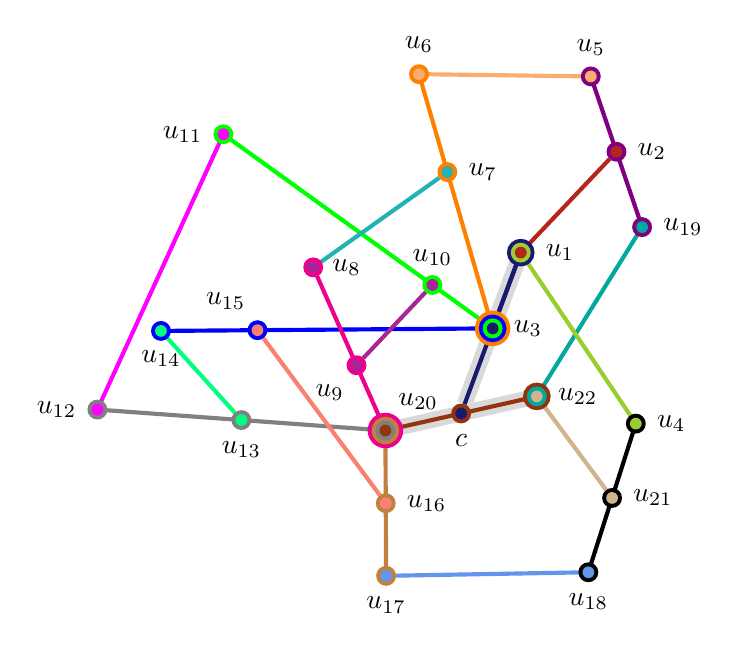
\begin{tikzpicture} [scale=0.5,rotate=0]

\tikzstyle{every path}=[line width=1.5pt]

\tikzstyle{c4}=[circle,inner sep=4pt,minimum size=7pt]
\tikzstyle{c3}=[circle,inner sep=3pt,minimum size=5pt]
\tikzstyle{c2}=[circle,inner sep=2pt,minimum size=3pt]
\tikzstyle{c1}=[circle,inner sep=1.5pt,minimum size=2pt]
\tikzstyle{c0}=[circle,inner sep=0.5pt,minimum size=1pt]

% Define positions of all observables

\path
( {4 *2.68838},{4 * 2.05247}) coordinate(1)
%( {4 *3.52352},{4 * 2.74293}) coordinate(2)
% ( {4 *1.15632},{4 * 2.50159}) coordinate(3)
( {4 *3.41896},{4 * 0.966553}) coordinate(4)
( {4 *3.13324},{4 * 3.17128}) coordinate(5)
( {4 *2.04217},{4 * 3.18563}) coordinate(6)
%( {4 *1.41836},{4 * 2.94988}) coordinate(7)
( {4 *1.37051},{4 * 1.95877}) coordinate(8)
%( {4 *0.727813},{4 * 1.89297}) coordinate(9)
%( {4 *0.284452},{4 * 2.64118}) coordinate(10)
( {4 *0.8},{4 * 2.80416}) coordinate(11)
( {4 *0.00},{4 * 1.05577}) coordinate(12)
%( {4 *0.352218},{4 * 0.592019}) coordinate(13)
( {4 *0.40372},{4 * 1.55514}) coordinate(14)
%( {4 *0.885362},{4 * 1.15654}) coordinate(15)
( {4 *1.26923},{4 * 0.189747}) coordinate(16)
( {4 *1.83338},{4 * 0.}) coordinate(17)
( {4 *3.11765},{4 * 0.0226601}) coordinate(18)
( {4 *3.45895},{4 * 2.21445}) coordinate(19)
( {4 *1.82887},{4 * 0.922707}) coordinate(20)
( {4 *3.58461},{4 * 0.431072}) coordinate(21)
( {4 *2.79057},{4 * 1.13936}) coordinate(22)
;

\draw [line width=2mm,color=gray!30] (20) -- (22);
\draw [color=RawSienna]   (20) -- (22) coordinate[c2,fill=RawSienna,draw=RawSienna,pos=0.5,label=270:{\color{black}$c$}] (31);
\draw [line width=2mm,color=gray!30] (1) -- (31);
\draw [color=MidnightBlue]   (1) -- (31) coordinate[c2,fill=MidnightBlue,draw=MidnightBlue,pos=0.5,label=0:{\color{black}$u_3$}] (3);
\draw [color=orange]    (3) -- (6) coordinate[c2,fill=orange,draw=orange,pos=0.6,label=0:{\color{black}$u_{7}$}] (7);
\draw [color=blue]    (3) -- (14) coordinate[c2,fill=blue,draw=blue,pos=0.7,label=95:{\color{black}$u_{15}$}] (15);
\draw [color=green]     (3) -- (11) coordinate[c2,fill=green,draw=green,pos=0.2] (10);
\draw [color=magenta]   (8) -- (20) coordinate[c2,fill=magenta,draw=magenta,pos=0.6] (9);
\draw [color=black]     (4) -- (18) coordinate[c2,fill=black,draw=black,pos=0.5,label=0:{\color{black}$u_{21}$}] (21);
\draw [color=brown]    (17) -- (20) coordinate[c2,fill=brown,draw=brown,pos=0.5,label=0:{\color{black}$u_{16}$}] (16);
\draw [color=gray]     (12) -- (20) coordinate[c2,fill=gray,draw=gray,pos=0.5,label=270:{\color{black}$u_{13}$}] (13);
\draw [color=violet]    (5) -- (19) coordinate[c2,fill=violet,draw=violet,pos=0.5,label=0:{\color{black}$u_{2}$}] (2);
\draw [color=Apricot]    (5) -- (6) ;
\draw [color=TealBlue]   (7) -- (8);
\draw [color=MidnightBlue]  (3) -- (1);
\draw [color=Mulberry]   (10) -- (9);
\draw [color=BrickRed]   (2) -- (1);
\draw [color=Emerald]    (19) -- (22);
\draw [color=YellowGreen]   (1) -- (4);
\draw [color=Tan]     (22) -- (21);
\draw [color=SpringGreen]   (14) -- (13);
\draw [color=Salmon]    (15) -- (16);
\draw [color=Fuchsia]    (11) -- (12);
\draw [color=CornflowerBlue]  (17) -- (18);

 \draw (10) coordinate[c1,fill=Mulberry,label=90:{\color{black}$u_{10}$}];
 \draw (13) coordinate[c1,fill=SpringGreen];
 \draw (15) coordinate[c1,fill=Salmon];
 \draw (9) coordinate[c1,fill=Mulberry,label=260:{\color{black}$u_{9}$}];
 \draw (7) coordinate[c1,fill=TealBlue];
 \draw (2) coordinate[c1,fill=BrickRed];
 \draw (21) coordinate[c1,fill=Tan];
 \draw (16) coordinate[c1,fill=Salmon];


 \draw (11) coordinate[c2,fill=green,draw=green,label=180:{\color{black}$u_{11}$}];
 %\draw (11) coordinate[c2,fill=YellowGreen,draw=YellowGreen];
 \draw (11) coordinate[c1,fill=Fuchsia];

 \draw (12) coordinate[c2,fill=gray,draw=gray,label=180:{\color{black}$u_{12}$}];
 \draw (12) coordinate[c1,fill=Fuchsia];

 \draw (14) coordinate[c2,fill=blue,draw=blue];
 \draw (14) coordinate[c1,fill=SpringGreen,label=270:{\color{black}$u_{14}$}];

 \draw (3) coordinate[c4,fill=orange,draw=orange];
 \draw (3) coordinate[c3,fill=blue,draw=blue];
 \draw (3) coordinate[c2,fill=green,draw=green];
 \draw (3) coordinate[c1,fill=MidnightBlue];


 \draw (20) coordinate[c4,fill=magenta,draw=magenta];
 \draw (20) coordinate[c3,fill=brown,draw=brown];
 \draw (20) coordinate[c2,fill=gray,draw=gray,label=80:{\color{black}$u_{20}$}];
 \draw (20) coordinate[c1,fill=RawSienna];

 \draw (6) coordinate[c2,fill=orange,draw=orange,label=90:{\color{black}$u_{6}$}];
 \draw (6) coordinate[c1,fill=Apricot];

 \draw (5) coordinate[c2,fill=violet,draw=violet,label=90:{\color{black}$u_{5}$}];
 \draw (5) coordinate[c1,fill=Apricot];

 \draw (19) coordinate[c2,fill=violet,draw=violet,label=0:{\color{black}$u_{19}$}];
 \draw (19) coordinate[c1,fill=Emerald];

 \draw (4) coordinate[c2,fill=black,draw=black,label=0:{\color{black}$u_{4}$}];
 \draw (4) coordinate[c1,fill=YellowGreen];

 \draw (18) coordinate[c2,fill=black,draw=black,label=270:{\color{black}$u_{18}$}];
 \draw (18) coordinate[c1,fill=CornflowerBlue];

 \draw (17) coordinate[c2,fill=brown,draw=brown,label=270:{\color{black}$u_{17}$}];
 \draw (17) coordinate[c1,fill=CornflowerBlue];

 \draw (8) coordinate[c2,fill=magenta,draw=magenta];
 \draw (8) coordinate[c1,fill=Mulberry,label=0:{\color{black}$u_{8}$}];


 \draw (1) coordinate[c3,fill=MidnightBlue,draw=MidnightBlue,label=0:{\color{black}$u_{1}$}];
 \draw (1) coordinate[c2,fill=violet,draw=YellowGreen];
 \draw (1) coordinate[c1,fill=BrickRed];

 \draw (22) coordinate[c3,fill=RawSienna,draw=RawSienna];
 \draw (22) coordinate[c2,fill=Emerald,draw=Emerald,label=0:{\color{black}$u_{22}$}];
 \draw (22) coordinate[c1,fill=Tan];

 \draw (31) coordinate[c1,fill=MidnightBlue];

\end{tikzpicture}
\end{center}
\caption{\label{2019-c-HH10}
Orthogonality hypergraph from a proof of
Theorem~3 in~\cite{Ramanathan-18}.
The advantage of this nonfull/TIFS/10-gadget
is a straightforward parametric faithful orthogonal representation allowing angles
$0< \angle u_1,u_{22} \le \frac{\pi}{4}$ radians ($45^\circ$)
of, say, the terminal points $u_1$ and $u_{22}$.
The corresponding logic including the completed set of
34~vertices in
21~blocks is set representable by partition logics because the supported 89~two-valued
states are (color) separable.
It is not too difficult to prove (by contradiction) that, say,
if both $u_1$, as well as $u_{22}$
are assumed to be one, then
$u_2$,
$u_3$,
$u_4$,
as well as
$u_{19}$,
$u_{20}$,
and $u_{21}$
should be zero.
Therefore,
$u_5$ and
$u_{18}$
would need to be true.
As a result,
$u_{6}$ and
$u_{17}$ would need to be false.
Hence,
$u_{7}$, as well as
$u_{16}$ would be one,
rendering
$u_{8}$ and
$u_{15}$ to be zero.
This would imply
$u_{9}$, as well as
$u_{14}$ to be one,
which in turn would demand
$u_{10}$ and
$u_{13}$ to be false.
Therefore,
$u_{11}$ and
$u_{12}$ would have to be one which yields a complete contradiction even for Type (III)
value assignments.
It is also a TITS/11-gadget for the terminal points
$u_1-u_{20}$, constructed by the standard construction depicted in~Figure~\ref{2018-c-fcloud10-11}.
}
\end{figure}

\section{Discussion}

It is important to notice that, for {fixed terminal vertices}, depending on the {cloud chosen}, very different classical predictions follow.
Indeed, once the terminal vertices are fixed, it is not too difficult to enumerate a quantum cloud that,
interpreted classically, predicts and demands {any} kind of input-output behavior.
This renders an element of arbitrariness in the interpretation of quantum~clouds.

The relevance of this observation lies in the conceivable interpretation of elementary empirical observations,
such as a single particular click in a detector.
Suppose a quantum is prepared in a pure state ``along'' a unit vector ${\bf a}$ and, when measured ``along''
$\textsf{\textbf{E}}_{\bf b}={\bf b}^\dagger {\bf b}$,
``happens to activate a detector'' corresponding to that state ${\bf b}$;
that is, a detector associated with this latter property clicks.
Depending on the quantum cloud considered, the following contradictory claims are justified:
\begin{enumerate}
\item
if the quantum cloud allows both values, then the claim is that there is no determination of the outcome; the event ``popped up'' from nowhere, {ex nihilo},
or, theologically speaking, has come about by {creatio continua} (cf. Kelly James Clark's God-as-Curler metaphor~\cite{Clark-2017-GodAsCurler});
\item
in the case of a 10-gadget, the system is truly quantum and cannot be classical;
\item
in the case of an 11-gadget, the system could be classical;
\item
in the case of a cloud inducing value indefiniteness, the claim can be justified that the system cannot be classical, as no such event (not even its absence)
should be recorded. Indeed, relative to the assumptions made, the (non)occurrence of any event at all is in contradiction to the classical~predictions.
\end{enumerate}

Conversely, if the experimenter observes no click in a detector associated with the state $ {\bf b} $,
then, depending on the quantum cloud considered, the following contradictory claims are justified:
\begin{enumerate}
\item
as mentioned earlier, if the quantum cloud allows both values, then there exists {creatio continua}
(currently, this appears to be the orthodox majority position);
\item
in the case of a 10-gadget, the system could be classical;
\item
in the case of an 11-gadget, the system is truly quantum and cannot be classical;
\item
just as mentioned earlier, in the case of a cloud inducing value indefiniteness, the claim can be justified that the system cannot be classical, as no such event (not even its absence)
should be recorded.
\end{enumerate}

As a result, depending on the quantum cloud considered, any (non)occurrence of some single outcome can be published
(or rather marketed in venerable scientific journals)
as a crucial experiment indicating that the associated system cannot be classical.
Likewise, by taking other quantum clouds, any such outcome may be considered to be consistent with classicality:
(non)classicality turns out to be {means relative} with respect to the quantum clouds considered.
As quantum clouds are configurable for any input-output port setup, this is true for any measurement outcome.


The situation turns even more precarious if one considers quantum clouds with a nonunital (and nonseparable) set of two-valued states,
such as the ones
depicted in Figures~\ref{2018-c-f-TIFS} and~\ref{2018-c-f-TITS}:
in the particular faithful orthogonal
representation~(\cite{2015-AnalyticKS}, Table~1, p.~102201-7),
the vector along
$\frac{1}{\sqrt{10}}\begin{pmatrix} 2\sqrt{2},1,-1 \end{pmatrix}$
yields a classical prediction amounting to the {nonoccurrence} of the particular
quantum observable. For another example,
take a cloud introduced by Tkadlec~(\cite{tkadlec-96}, Figure~2).
It is based on a set of orthogonal vectors
communicated to Specker by Sch\"utte~\cite{clavadetscher} and contains
36~vertices in 26~contexts/cliques, which allow six~two-valued states
enforcing eight~vertices to be zero. In the particular faithful orthogonal representation of Tkadlec,
those correspond to the vectors along
$\begin{pmatrix} 1,0,0 \end{pmatrix}$,
$\begin{pmatrix} 0,0,1 \end{pmatrix}$,
$\begin{pmatrix} 1,0,1 \end{pmatrix}$,
$\begin{pmatrix} 1,0,-1 \end{pmatrix}$,
$\begin{pmatrix} 2,0,-1 \end{pmatrix}$,
$\begin{pmatrix} 1,0,2 \end{pmatrix}$,
$\begin{pmatrix} -1,0,2 \end{pmatrix}$, and
$\begin{pmatrix} 2,0,1 \end{pmatrix}$.
At the same time, the vector
$\begin{pmatrix} 0,1,0 \end{pmatrix}$ is forced to be one.
Since without loss of generality, an orthogonal transformation can transform all of
these vectors into other arbitrary directions (while maintaining the angles between vectors and,
in particular, orthogonality),
the assumption of such unital configurations
and their classical interpretation
immediately yields any desired contradiction
with any individual measurement outcome.

This arbitrariness could be overcome by some sort of ``superselection rule''
prioritizing or selecting particular quantum clouds over other ones.
However, in the absence of such superselection rules, a generalized Jayne's principle, or rather Laplace's principle of indifference,
implies that any choice of a particular quantum cloud over other ones
amounts to an ``epistemic massaging'' of empirical data and their nonoperational,
misleading overinterpretation in terms of a speculative ontology~\cite{berkeley,stace,Goldschmidt2017-idealism};
or, to quote Peres~\cite{peres222}, {``unperformed experiments have no results''.}
In contradistinction, it may not be too speculative to hold it for granted that the only operationally
justified ontology is the assumption of a single one context or its associated maximal observable.%missing the Conclusions?

%%% \begin{acknowledgments}
%%% I kindly acknowledge enlightening discussions with Adan Cabello, Jos\'{e} R. Portillo, and Mohammad Hadi Shekarriz.
%%% I am grateful to Josef Tkadlec for providing a {\em Pascal} program
%%% which computes and analyses the set of two-valued states of collections of contexts.
%%% All misconceptions and errors are mine.
%%% \end{acknowledgments}


\funding{The author acknowledges the support by the Austrian Science Fund (FWF): Project I 4579-N, and the Czech Science Foundation (GA\v CR): Project 20-09869L.}

%%%%%%%%%%%%%%%%%%%%%%%%%%%%%%%%%%%%%%%%%%
\acknowledgments{I kindly acknowledge enlightening discussions with Adan Cabello, Jos\'{e} R. Portillo, and~Mohammad Hadi Shekarriz.
I am grateful to Josef Tkadlec for providing a {Pascal} program,
which computes and~analyses the set of two-valued states of collections of contexts.
All misconceptions and errors are mine.
}

%%%%%%%%%%%%%%%%%%%%%%%%%%%%%%%%%%%%%%%%%%
\conflictsofinterest{The author declares no conflict of interest.}


%%%%%%%%%%%%%%%%%%%%%%%%%%%%%%%%%%%%%%%%%%
\reftitle{References}

% Please provide either the correct journal abbreviation (e.g. according to the “List of Title Word Abbreviations” http://www.issn.org/services/online-services/access-to-the-ltwa/) or the full name of the journal.
% Citations and References in Supplementary files are permitted provided that they also appear in the reference list here.

%=====================================
% References, variant A: external bibliography
%=====================================
%\externalbibliography{yes}

%\bibliography{svozil}
%%% \bibliographystyle{apsrev}


\begin{thebibliography}{999}
\providecommand{\natexlab}[1]{#1}

\bibitem[{von Neumann}(1932, 1996)]{v-neumann-49}
{von Neumann}, J.
\newblock {\em {M}athematische {G}rundlagen der {Q}uantenmechanik}, 2nd ed.;
 Springer: Berlin/Heidelberg, Germany,  1932, 1996,
 doi:{\changeurlcolor{black}\href{https://doi.org/10.1007/978-3-642-61409-5}{\detokenize{10.1007/978-3-642-61409-5}}}. % please confirm the year information

\bibitem[{von Neumann}(1955)]{v-neumann-55}
{von Neumann}, J.
\newblock {\em Mathematical Foundations of Quantum Mechanics}; Princeton
 University Press: Princeton,~NJ,~USA, 1955.

\bibitem[Birkhoff and {von Neumann}(1936)]{birkhoff-36}
Birkhoff, G.; {von Neumann}, J.
\newblock The Logic of Quantum Mechanics.
\newblock {\em Ann. Math.} {\bf 1936}, {\em 37},~823--843,
\newblock
 doi:{\changeurlcolor{black}\href{https://doi.org/10.2307/1968621}{\detokenize{10.2307/1968621}}}.

\bibitem[{Everett III}(1957)]{everett}
{Everett III}, H.
\newblock `{R}elative {S}tate' Formulation of Quantum Mechanics.
\newblock {\em Rev. Mod. Phys.} {\bf 1957}, {\em 29},~454--462,
\newblock
 doi:{\changeurlcolor{black}\href{https://doi.org/10.1103/RevModPhys.29.454}{\detokenize{10.1103/RevModPhys.29.454}}}.

\bibitem[Wigner(1961,1962)]{wigner:mb}
Wigner, E.P.
\newblock Remarks on the mind-body question. In {\em The Scientist Speculates};
 Good, I.J., Ed.; Heinemann and Basic Books: London, UK, 1961; New York, NY, USA, 1962; Springer-Verlag, Berlin, 1995;
 pp. 284--302.
\newblock
 doi:{\changeurlcolor{black}\href{https://doi.org/10.1007/978-3-642-78374-6\_20}{\detokenize{10.1007/978-3-642-78374-6\_20}}}.

\bibitem[{Everett III}(1956,2012)]{everett-1956}
{Everett}, H, III.
\newblock The Theory of the Universal Wave Function. In {\em The {E}verett
 Interpretation of Quantum Mechanics: Collected Works 1955-1980 with
 Commentary}; Barrett, J.A.; Byrne, P., Eds.; Princeton University Press:
 Princeton, NJ, USA, 1956, 2012; pp. 72--172.

\bibitem[Berkeley(1710)]{berkeley}
Berkeley, G.
\newblock {\em A Treatise Concerning the Principles of Human Knowledge}; Aaron Rhames for Jeremy Pepyat, Bookseller: Skinner--Row, Dublin, 1710.

\bibitem[Stace(1934)]{stace}
Stace, W.T.
\newblock The Refutation of Realism.
\newblock {\em Mind} {\bf 1934}, {\em 43},~145--155,
\newblock
 doi:{\changeurlcolor{black}\href{https://doi.org/10.1093/mind/XLIII.170.145}{\detokenize{10.1093/mind/XLIII.170.145}}}.

\bibitem[Kochen and Specker(1965{\natexlab{a}})]{Kochen2}
Kochen, S.; Specker, E.P.
\newblock Logical Structures arising in quantum theory.
\newblock In \emph{The Theory of Models: Proceedings of the 1963 International
 Symposium at Berkeley}; North Holland: Amsterdam, The Netherlands; New York,~NY, USA; Oxford, UK, 1965; pp.
 177--189.

\bibitem[Kochen and Specker(1965{\natexlab{b}})]{Kochen3}
Kochen, S.; Specker, E.P.
\newblock The calculus of partial propositional functions.
\newblock In \emph{Proceedings of the 1964 International Congress for Logic,
 Methodology and Philosophy of Science, Jerusalem}; North Holland: Amsterdam,~The~Netherlands
 1965; pp. 45--57.

\bibitem[Abbott \em{et~al.}(2012)Abbott, Calude, Conder, and
 Svozil]{2012-incomput-proofsCJ}
Abbott, A.A.; Calude, C.S.; Conder, J.; Svozil, K.
\newblock Strong {K}ochen-{S}pecker theorem and incomputability of quantum
 randomness.
\newblock {\em Phys. Rev. A} {\bf 2012}, {\em 86},~062109.

\bibitem[Abbott \em{et~al.}(2015)Abbott, Calude, and Svozil]{2015-AnalyticKS}
Abbott, A.A.; Calude, C.S.; Svozil, K.
\newblock A variant of the {K}ochen-{S}pecker theorem localising value
 indefiniteness.
\newblock {\em J. Math. Phys.} {\bf 2015}, {\em
 56},~102201.

\bibitem[Kleene(1936)]{Kleene1936}
Kleene, S.C.
\newblock General recursive functions of natural numbers.
\newblock {\em Math. Ann.} {\bf 1936}, {\em 112},~727--742.

 \bibitem[Cabello \em{et~al.}(2018)Cabello, Portillo, Sol\'{i}s, and
 Svozil]{2018-minimalYIYS}
Cabello, A.; Portillo, J.R.; Sol\'{i}s, A.; Svozil, K.
\newblock Minimal true-implies-false and true-implies-true sets of propositions
 in noncontextual hidden-variable theories.
\newblock {\em Phys. Rev. A} {\bf 2018}, {\em 98},~012106.

\bibitem[Quisquater \em{et~al.}(1990)Quisquater, Quisquater, Quisquater,
 Quisquater, Guillou, Guillou, Guillou, Guillou, Guillou, and
 Guillou]{Quisquater1990}
Quisquater, J.J.; Quisquater, M.; Quisquater, M.; Quisquater, M.; Guillou, L.;
 Guillou, M.A.; Guillou, G.; Guillou, A.; Guillou, G.; Guillou, S.
\newblock How to Explain Zero-Knowledge Protocols to Your Children.
\newblock In~Advances in Cryptology---CRYPTO' 89 Proceedings; Brassard, G., Ed.;
 Springer: New York, NY, USA, 1990; pp. 628--631,
\newblock
 doi:{\changeurlcolor{black}\href{https://doi.org/10.1007/0-387-34805-0\_60}{\detokenize{10.1007/0-387-34805-0\_60}}}.

\bibitem[Specker(1960)]{Specker-60}
Specker, E.
\newblock {D}ie {L}ogik nicht gleichzeitig entscheidbarer {A}ussagen.
\newblock {\em Dialectica} {\bf 1960}, {\em 14},~239--246.

\bibitem[Goldschmidt and Pearce(2017, 2018)]{Goldschmidt2017-idealism}
Goldschmidt, T.; Pearce, K.L.
\newblock {\em Idealism: New Essays in Metaphysics}; Oxford University Press:
 Oxford, UK,  2017, 2018,
\newblock
 doi:{\changeurlcolor{black}\href{https://doi.org/10.1093/oso/9780198746973.001.0001}{\detokenize{10.1093/oso/9780198746973.001.0001}}}.

\bibitem[Bridgman(1934)]{bridgman}
Bridgman, P.W.
\newblock A Physicist's Second Reaction to {M}engenlehre.
\newblock {\em Scr. Math.} {\bf 1934}, {\em 2},~101--117, 224--234.

\bibitem[Kochen and Specker(1967)]{Kochen1}
Kochen, S.; Specker, E.P.
\newblock The Problem of Hidden Variables in Quantum Mechanics.
\newblock {\em J. Math. Mech.} {\bf 1967}, {\em 17},~59--87.

\bibitem[Svozil(2005)]{svozil-2001-eua}
Svozil, K.
\newblock Logical equivalence between generalized urn models and finite
 automata.
\newblock {\em Int. J. Theor. Phys.} {\bf 2005}, {\em
 44},~745--754.

\bibitem[Moore(1956)]{e-f-moore}
Moore, E.F.
\newblock Gedanken-Experiments on Sequential Machines. In {\em Automata
 Studies {(AM-34)}}; Shannon, C.E., McCarthy, J., Eds.; Princeton University
 Press: Princeton, NJ, USA, 1956; pp. 129--153.

\bibitem[Wright(1978)]{wright:pent}
Wright, R.
\newblock The state of the pentagon. {A} nonclassical example. In {\em
 Mathematical Foundations of Quantum Theory}; Marlow, A.R., Ed.; Academic
 Press: New York, NY, USA, 1978; pp. 255--274.

\bibitem[Wright(1990)]{wright}
Wright, R.
\newblock Generalized urn models.
\newblock {\em Found. Phys.} {\bf 1990}, {\em 20},~881--903,
\newblock
 doi:{\changeurlcolor{black}\href{https://doi.org/10.1007/BF01889696}{\detokenize{10.1007/BF01889696}}}.

\bibitem[Gleason(1957)]{Gleason}
Gleason, A.M.
\newblock Measures on the closed subspaces of a {H}ilbert space.
\newblock {\em J. Math. Mech.} {\bf 1957}, {\em 6},~885--893.
\newblock
 doi:{\changeurlcolor{black}\href{https://doi.org/10.1512/iumj.1957.6.56050}{\detokenize{10.1512/iumj.1957.6.56050}}}.

\bibitem[Godsil and Newman(2008)]{Godsil-Newman-2008}
Godsil, C.D.; Newman, M.W.
\newblock Coloring an Orthogonality Graph.
\newblock {\em SIAM J. Discret. Math.} {\bf 2008}, {\em
 22},~683--692.

\bibitem[Halmos(1958)]{halmos-vs}
Halmos, P.R.
\newblock {\em Finite-Dimensional Vector Spaces}; Undergraduate Texts in
 Mathematics. Springer: New~York,~NY,~USA, 1958.

\bibitem[Lov\'asz \em{et~al.}(1989)Lov\'asz, Saks, and Schrijver]{lovasz-89}
Lov\'asz, L.; Saks, M.; Schrijver, A.
\newblock Orthogonal representations and connectivity of graphs.
\newblock {\em Linear Algebra Its Appl.} {\bf 1989}, {\em
 114},~439--454.

\bibitem[Sol\'is-Encina and Portillo(2015)]{Portillo-2015}
Sol\'is-Encina, A.; Portillo, J.R.
\newblock Orthogonal Representation of Graphs. {\em arXiv} \textbf{2015}, arXiv:1504.03662.

\bibitem[Greechie(1971)]{greechie:71}
Greechie, R.J.
\newblock Orthomodular lattices admitting no states.
\newblock {\em J. Comb. Theory Ser. A} {\bf 1971}, {\em
 10},~119--132,
\newblock
 doi:{\changeurlcolor{black}\href{https://doi.org/10.1016/0097-3165(71)90015-X}{\detokenize{10.1016/0097-3165(71)90015-X}}}.

\bibitem[Navara and Rogalewicz(1991)]{nav:91}
Navara, M.; Rogalewicz, V.
\newblock The pasting constructions for orthomodular posets.
\newblock {\em Math. Nachr.} {\bf 1991},~{\em 154},~157--168,
\newblock
 doi:{\changeurlcolor{black}\href{https://doi.org/10.1002/mana.19911540113}{\detokenize{10.1002/mana.19911540113}}}.

\bibitem[Reck \em{et~al.}(1994)Reck, Zeilinger, Bernstein, and Bertani]{rzbb}
Reck, M.; Zeilinger, A.; Bernstein, H.J.; Bertani, P.
\newblock Experimental realization of any discrete unitary operator.
\newblock {\em Phys. Rev. Lett.} {\bf 1994},~{\em 73},~58--61,
\newblock
 doi:{\changeurlcolor{black}\href{https://doi.org/10.1103/PhysRevLett.73.58}{\detokenize{10.1103/PhysRevLett.73.58}}}.

\bibitem[Cabello(2008)]{cabello:210401}
Cabello, A.
\newblock Experimentally Testable State-Independent Quantum Contextuality.
\newblock {\em Phys. Rev. Lett.} {\bf 2008},~{\em 101},~210401.

\bibitem[Pitowsky(1998)]{pitowsky:218}
Pitowsky, I.
\newblock Infinite and finite {G}leason's theorems and the logic of
 indeterminacy.
\newblock {\em J. Math. Phys.} {\bf 1998},~{\em 39},~218--228,
\newblock
 doi:{\changeurlcolor{black}\href{https://doi.org/10.1063/1.532334}{\detokenize{10.1063/1.532334}}}.

\bibitem[Abbott \em{et~al.}(2014)Abbott, Calude, and
 Svozil]{PhysRevA.89.032109}
Abbott, A.A.; Calude, C.S.; Svozil, K.
\newblock Value-indefinite observables are almost everywhere.
\newblock {\em Phys. Rev. A} {\bf 2014},~{\em 89},~032109.

\bibitem[Svozil and Tkadlec(1996)]{svozil-tkadlec}
Svozil, K.; Tkadlec, J.
\newblock Greechie diagrams, nonexistence of measures in quantum logics and
 {K}ochen--{S}pecker type constructions.
\newblock {\em J. Math. Phys.} {\bf 1996}, {\em
 37},~5380--5401,
\newblock
 doi:{\changeurlcolor{black}\href{https://doi.org/10.1063/1.531710}{\detokenize{10.1063/1.531710}}}.

\bibitem[Tkadlec(1998)]{tkadlec-96}
Tkadlec, J.
\newblock {G}reechie diagrams of small quantum logics with small state spaces.
\newblock {\em Int. J. Theor. Phys.} {\bf 1998}, {\em
 37},~203--209.
\newblock
 doi:{\changeurlcolor{black}\href{https://doi.org/10.1023/A:1026646229896}{\detokenize{10.1023/A:1026646229896}}}.

\bibitem[Boole(1862)]{Boole-62}
Boole, G.
\newblock On the Theory of Probabilities.
\newblock {\em Philos. Trans. R. Soc. Lond.} {\bf
 1862}, {\em 152},~225--252.
\newblock
 doi:{\changeurlcolor{black}\href{https://doi.org/10.1098/rstl.1862.0015}{\detokenize{10.1098/rstl.1862.0015}}}.

\bibitem[Froissart(1981)]{froissart-81}
Froissart, M.
\newblock Constructive generalization of {B}ell's inequalities.
\newblock {\em Il Nuovo Cim. B (1971--1996)} {\bf 1981}, {\em 64},~241--251.
\newblock 10.1007/BF02903286.

\bibitem[{Cirel'son (=Tsirel'son)}(1993)]{cirelson}
{Tsirelson}, B.S.
\newblock Some results and problems on quantum {B}ell-type inequalities.
\newblock {\em Hadron. J. Suppl.} {\bf 1993},~{\em 8},~329--345.

\bibitem[Pitowsky(1986)]{pitowsky-86}
Pitowsky, I.
\newblock The range of quantum probabilities.
\newblock {\em J. Math. Phys.} {\bf 1986}, {\em
 27},~1556--1565.

\bibitem[Pitowsky(1989{\natexlab{a}})]{pitowsky}
Pitowsky, I.
\newblock Quantum Probability---Quantum Logic. In {\em Lecture
 Notes in Physics}; Springer: Berlin/Heidelberg, Germany, 1989; Volume 321.

\bibitem[Pitowsky(1989{\natexlab{b}})]{pitowsky-89a}
Pitowsky, I.
\newblock From {G}eorge {B}oole to {J}ohn {B}ell: The origin of {B}ell's
 inequality. In {\em {B}ell's Theorem, Quantum Theory and the Conceptions of
 the Universe}; Fundamental Theories of
 Physics; Kafatos, M., Ed.; Kluwer Academic Publishers, Springer: Dordrecht, The Netherlands, 1989; Volume~37, pp. 37--49.
\newblock
 doi:{\changeurlcolor{black}\href{https://doi.org/10.1007/978-94-017-0849-4\_6}{\detokenize{10.1007/978-94-017-0849-4\_6}}}.

\bibitem[Pitowsky(1991)]{Pit-91}
Pitowsky, I.
\newblock Correlation polytopes their geometry and complexity.
\newblock {\em Math. Program.} {\bf 1991}, {\em 50},~395--414.
\newblock
 doi:{\changeurlcolor{black}\href{https://doi.org/10.1007/BF01594946}{\detokenize{10.1007/BF01594946}}}.

\bibitem[Pitowsky(1994)]{Pit-94}
Pitowsky, I.
\newblock {G}eorge {B}oole's `Conditions of Possible Experience' and the
 Quantum Puzzle.
\newblock {\em Br. J. Philos. Sci.} {\bf 1994},
 {\em 45},~95--125,
\newblock
 doi:{\changeurlcolor{black}\href{https://doi.org/10.1093/bjps/45.1.95}{\detokenize{10.1093/bjps/45.1.95}}}.

\bibitem[Pitowsky and Svozil(2001)]{2000-poly}
Pitowsky, I.; Svozil, K.
\newblock New optimal tests of quantum nonlocality.
\newblock {\em Phys. Rev. A} {\bf 2001}, {\em 64},~014102.

\bibitem[Svozil(2012)]{svozil-2011-enough}
Svozil, K.
\newblock How much contextuality?
\newblock {\em Nat. Comput.} {\bf 2012}, {\em 11},~261--265,

\bibitem[Zierler and Schlessinger(1975)]{Zierler1975}
Zierler, N.; Schlessinger, M.
\newblock Boolean Embeddings of Orthomodular Sets and Quantum Logic.
\newblock In {\em The Logico-Algebraic Approach to Quantum Mechanics: Volume I:
 Historical Evolution}; Hooker, C.A., Ed.; Springer: Dordrecht, The Netherlands
 1975; pp. 247--262.
\newblock
 doi:{\changeurlcolor{black}\href{https://doi.org/10.1007/978-94-010-1795-4_14}{\detokenize{10.1007/978-94-010-1795-4_14}}}.

\bibitem[Tutte(1954)]{tutte_1954}
Tutte, W.T.
\newblock A Short Proof of the Factor Theorem for Finite Graphs.
\newblock {\em Can. J. Math.} {\bf 1954}, {\em 6},~347--352,
\newblock
 doi:{\changeurlcolor{black}\href{https://doi.org/10.4153/CJM-1954-033-3}{\detokenize{10.4153/CJM-1954-033-3}}}.

\bibitem[Szab\'o(2009)]{SZABO2009436}
Szab\'o, J.
\newblock Good characterizations for some degree constrained subgraphs.
\newblock {\em J. Comb. Theory Ser. B} {\bf 2009}, {\em
 99},~436--446,
\newblock
 doi:{\changeurlcolor{black}\href{https://doi.org/10.1016/j.jctb.2008.08.009}{\detokenize{10.1016/j.jctb.2008.08.009}}}.

\bibitem[Ramanathan \em{et~al.}(2018)Ramanathan, Rosicka, Horodecki, Pironio,
 Horodecki, and Horodecki]{Ramanathan-18}
Ramanathan, R.; Rosicka, M.; Horodecki, K.; Pironio, S.; Horodecki, M.;
 Horodecki, P.
\newblock Gadget structures in proofs of the {K}ochen-{S}pecker theorem. \emph{arXiv} \textbf{2018}, arXiv:1807.00113.

\bibitem[Svozil(2018)]{svozil-2016-pu-book}
Svozil, K.
\newblock {\em Physical [A]Causality. {D}eterminism, Randomness and Uncaused
 Events}; Springer: Cham, Switzerland; Berlin/Heidelberg, Germany; New York, NY, USA, 2018.
\newblock
 doi:{\changeurlcolor{black}\href{https://doi.org/10.1007/978-3-319-70815-7}{\detokenize{10.1007/978-3-319-70815-7}}}.

\bibitem[Svozil(2009)]{svozil-2006-omni}
Svozil, K.
\newblock Quantum Scholasticism: On Quantum Contexts, Counterfactuals, and the
 Absurdities of Quantum Omniscience.
\newblock {\em Inf. Sci.} {\bf 2009}, {\em 179},~535--541,
\newblock
 doi:{\changeurlcolor{black}\href{https://doi.org/10.1016/j.ins.2008.06.012}{\detokenize{10.1016/j.ins.2008.06.012}}}.

\bibitem[Cohen(1989)]{cohen}
Cohen, D.W.
\newblock {\em An Introduction to Hilbert Space and Quantum Logic}; Problem
 Books in Mathematics; Springer: New York, NY, USA, 1989.
\newblock
 doi:{\changeurlcolor{black}\href{https://doi.org/10.1007/978-1-4613-8841-8}{\detokenize{10.1007/978-1-4613-8841-8}}}.

\bibitem[Stairs(1983)]{stairs83}
Stairs, A.
\newblock Quantum logic, realism, and value definiteness.
\newblock {\em Philos. Sci.} {\bf 1983}, {\em 50},~578--602,
\newblock
 doi:{\changeurlcolor{black}\href{https://doi.org/10.1086/289140}{\detokenize{10.1086/289140}}}.

\bibitem[Yu and Oh(2012)]{Yu-2012}
Yu, S.; Oh, C.H.
\newblock State-Independent Proof of {K}ochen-{S}pecker Theorem with 13 Rays.
\newblock {\em Phys. Rev. Lett.} {\bf 2012},~{\em 108},~030402,

\bibitem[Clifton(1993)]{clifton-93}
Clifton, R.K.
\newblock Getting contextual and nonlocal elements-of-reality the easy way.
\newblock {\em Am. J. Phys.} {\bf 1993}, {\em 61},~443--447.
\newblock
 doi:{\changeurlcolor{black}\href{https://doi.org/10.1119/1.17239}{\detokenize{10.1119/1.17239}}}.

\bibitem[Belinfante(1973)]{Belinfante-73}
Belinfante, F.J.
\newblock A Survey of Hidden-Variables Theories. In {\em
 International Series of Monographs in Natural Philosophy}; Pergamon Press: Oxford, UK; Elsevier: New York, NY, USA, 1973; Volume~55.
\newblock
 doi:{\changeurlcolor{black}\href{https://doi.org/10.1016/B978-0-08-017032-9.50001-7}{\detokenize{10.1016/B978-0-08-017032-9.50001-7}}}.

\bibitem[Pitowsky(1982)]{Pitowsky-1982-subs}
Pitowsky, I.
\newblock Substitution and Truth in Quantum Logic.
\newblock {\em Philos. Sci.} {\bf 1982}, {\em 49},~380--401.
\newblock
 doi:{\changeurlcolor{black}\href{https://doi.org/10.2307/187281}{\detokenize{10.2307/187281}}}.

\bibitem[Hardy(1992)]{Hardy-92}
Hardy, L.
\newblock Quantum mechanics, local realistic theories, and Lorentz-invariant
 realistic theories.
\newblock {\em Phys.~Rev.~Lett.} {\bf 1992}, {\em 68},~2981--2984.
\newblock
 doi:{\changeurlcolor{black}\href{https://doi.org/10.1103/PhysRevLett.68.2981}{\detokenize{10.1103/PhysRevLett.68.2981}}}.

\bibitem[Hardy(1993)]{Hardy-93}
Hardy, L.
\newblock Nonlocality for two particles without inequalities for almost all
 entangled states.
\newblock {\em Phys. Rev. Lett.} {\bf 1993}, {\em 71},~1665--1668.
\newblock
 doi:{\changeurlcolor{black}\href{https://doi.org/10.1103/PhysRevLett.71.1665}{\detokenize{10.1103/PhysRevLett.71.1665}}}.

\bibitem[Boschi \em{et~al.}(1997)Boschi, Branca, De~Martini, and
 Hardy]{hardy-97}
Boschi, D.; Branca, S.; De~Martini, F.; Hardy, L.
\newblock Ladder Proof of Nonlocality without Inequalities: Theoretical and
 Experimental Results.
\newblock {\em Phys. Rev. Lett.} {\bf 1997}, {\em 79},~2755--2758.
\newblock
 doi:{\changeurlcolor{black}\href{https://doi.org/10.1103/PhysRevLett.79.2755}{\detokenize{10.1103/PhysRevLett.79.2755}}}.

\bibitem[Cabello and Garc{\'{i}}a-Alcaine(1995)]{Cabello-1995-ppks}
Cabello, A.; Garc{\'{i}}a-Alcaine, G.
\newblock A hidden-variables versus quantum mechanics experiment.
\newblock {\em J. Phys. A Math. Gen. Phys.} {\bf
 1995}, {\em 28},~3719--3724.
\newblock
 doi:{\changeurlcolor{black}\href{https://doi.org/10.1088/0305-4470/28/13/016}{\detokenize{10.1088/0305-4470/28/13/016}}}.

\bibitem[Cabello \em{et~al.}(1996)Cabello, Estebaranz, and
 Garc{\'{i}}a-Alcaine]{cabello-96}
Cabello, A.; Estebaranz, J.M.; Garc{\'{i}}a-Alcaine, G.
\newblock {B}ell-{K}ochen-{S}pecker theorem: A proof with 18 vectors.
\newblock {\em Phys. Lett. A} {\bf 1996}, {\em 212},~183--187.

\bibitem[Cabello(1997)]{cabello-97-nhvp}
Cabello, A.
\newblock No-hidden-variables proof for two spin- particles preselected and
 postselected in unentangled states.
\newblock {\em Phys. Rev. A} {\bf 1997}, {\em 55},~4109--4111.
\newblock
 doi:{\changeurlcolor{black}\href{https://doi.org/10.1103/PhysRevA.55.4109}{\detokenize{10.1103/PhysRevA.55.4109}}}.

\bibitem[Badzi\c{a}g \em{et~al.}(2011)Badzi\c{a}g, Bengtsson, Cabello,
 Granstr\"om, and Larsson]{Badziag-2011}
Badzi\c{a}g, P.; Bengtsson, I.; Cabello, A.; Granstr\"om, H.; Larsson, J.A.
\newblock Pentagrams and Paradoxes.
\newblock {\em Found. Phys.} {\bf 2011}, {\em 41},~414--423,
\newblock
 doi:{\changeurlcolor{black}\href{https://doi.org/10.1007/s10701-010-9433-3}{\detokenize{10.1007/s10701-010-9433-3}}}.

\bibitem[Chen \em{et~al.}(2013)Chen, Cabello, Xu, Su, Wu, and
 Kwek]{Cabello-2013-HP}
Chen, J.L.; Cabello, A.; Xu, Z.P.; Su, H.Y.; Wu, C.; Kwek, L.C.
\newblock Hardy's paradox for high-dimensional systems.
\newblock {\em Phys. Rev. A} {\bf 2013}, {\em 88},~062116.
\newblock
 doi:{\changeurlcolor{black}\href{https://doi.org/10.1103/PhysRevA.88.062116}{\detokenize{10.1103/PhysRevA.88.062116}}}.

\bibitem[Cabello \em{et~al.}(2013)Cabello, Badziag, Terra~Cunha, and
 Bourennane]{Cabello-2013-Hardylike}
Cabello, A.; Badziag, P.; Terra~Cunha, M.; Bourennane, M.
\newblock Simple {H}ardy-Like Proof of Quantum Contextuality.
\newblock {\em Phys. Rev. Lett.} {\bf 2013}, {\em 111},~180404.
\newblock
 doi:{\changeurlcolor{black}\href{https://doi.org/10.1103/PhysRevLett.111.180404}{\detokenize{10.1103/PhysRevLett.111.180404}}}.

\bibitem[Dvure{\v{c}}enskij \em{et~al.}(1995)Dvure{\v{c}}enskij,
 Pulmannov{\'{a}}, and Svozil]{dvur-pul-svo}
Dvure{\v{c}}enskij, A.; Pulmannov{\'{a}}, S.; Svozil, K.
\newblock Partition Logics, Orthoalgebras and Automata.
\newblock {\em Helv. Phys. Acta} {\bf 1995}, {\em 68},~407--428.

\bibitem[Cabello(1994)]{cabello-1994}
Cabello, A.
\newblock A simple proof of the {K}ochen-{S}pecker theorem.
\newblock {\em Eur. J. Phys.} {\bf 1994}, {\em 15},~179--183.
\newblock
 doi:{\changeurlcolor{black}\href{https://doi.org/10.1088/0143-0807/15/4/004}{\detokenize{10.1088/0143-0807/15/4/004}}}.

\bibitem[Cabello(1996)]{Cabello-1996-diss}
Cabello, A.
\newblock Pruebas Algebraicas de Imposibilidad de Variables Ocultas en
 Mec{\'a}nica Cu{\'a}ntica.
\newblock Ph.D. Thesis, Universidad Complutense de Madrid, Madrid, Spain, 1996.

\bibitem[Svozil(2018)]{svozil-2018-whycontexts}
Svozil, K.
\newblock New Forms of Quantum Value Indefiniteness Suggest That Incompatible
 Views on Contexts Are Epistemic.
\newblock {\em Entropy} {\bf 2018}, {\em 20},~406.

\bibitem[Johansen(1994)]{Johansen-1994}
Johansen, H.B.
\newblock  Comment on ``Getting contextual and nonlocal elements-of-reality the
 easy way''.
\newblock {\em Am. J. Phys.} {\bf 1994}, {\em 62},~471.
\newblock
 doi:{\changeurlcolor{black}\href{https://doi.org/10.1119/1.17551}{\detokenize{10.1119/1.17551}}}.

\bibitem[Vermaas(1994)]{Vermaas-1994}
Vermaas, P.E.
\newblock  Comment on ``Getting contextual and nonlocal elements-of-reality the
 easy way''.
\newblock {\em Am. J.~Phys.} {\bf 1994}, {\em 62},~658.
\newblock
 doi:{\changeurlcolor{black}\href{https://doi.org/10.1119/1.17488}{\detokenize{10.1119/1.17488}}}. % please check ref.72 and ref.73

\bibitem[Svozil(2018)]{svozil-pac}
Svozil, K.
\newblock {\em Physical (A)Causality}; Fundamental Theories of
 Physics; Springer International Publishing: Cham,~Switzerland; Heidelberg, Germany; New York, NY, USA;
 Dordrecht, The Netherlands; London, UK, 2018; Volume 192.
\newblock
 doi:{\changeurlcolor{black}\href{https://doi.org/10.1007/978-3-319-70815-7}{\detokenize{10.1007/978-3-319-70815-7}}}. % please confirm the title information

\bibitem[Portillo(2018)]{Portillo-2018-pc}
Portillo, J.R.
\newblock Logical equivalence of nonseparability and ``true if and only if'' (TIFFTS). Private Conversation. % please add author's affiliation information and Title of unpublished work.
Universidad de Sevilla, Seville, Spain, 2018.

\bibitem[Clark(2017)]{Clark-2017-GodAsCurler}
Clark, K.J.
\newblock Is {G}od a Bowler or a Curler? 2017.
\newblock Presentation at the Randomness and Providence Workshop. 9~May 2017;
Kalamazoo, Michigan, USA, 2017.

\bibitem[Clavadetscher-Seeberger(1983)]{clavadetscher}
Clavadetscher-Seeberger, E.
\newblock Eine partielle Pr{\"{a}}dikatenlogik.
\newblock Ph.D. Thesis, ETH-Z{\"{u}}rich, Z{\"{u}}rich,~Switzerland,~1983.

\bibitem[Peres(1978)]{peres222}
Peres, A.
\newblock Unperformed experiments have no results.
\newblock {\em Am. J. Phys.} {\bf 1978}, {\em 46},~745--747.
\newblock
 doi:{\changeurlcolor{black}\href{https://doi.org/10.1119/1.11393}{\detokenize{10.1119/1.11393}}}.

\end{thebibliography}

%%%%%%%%%%%%%%%%%%%%%%%%%%%%%%%%%%%%%%%%%%
\end{document}

%%%%%%%%%%%%%%%%%%%%%%%%%%%%%%%%%%%%%%%%%%%%%%%%%%%%%%%%%%%%%%%%%%%%%%%%%%%%%%%%%%%%%%%%%%%%%%%%%%%%%%%%%%%%%%%%%%%%%%%%%%%%%%%%%%%%%%%%%%


va = {1,0,0} ;
vb = {Sqrt[2],1,1} ;
v1 = {0,1,1} ;
v2 = {0,1,-1} ;
v3 = {Sqrt[2],-1,-1} ;
v4 = {0,0,1} ;
v5 = {0,1,0} ;
v6 = {Sqrt[2],1,-3} ;
v7 = {1,-Sqrt[2],0} ;
v8 = {Sqrt[2],-3,1} ;
v9 = {1,0,-Sqrt[2]} ;
v10= {Sqrt[2],1,0} ;
v11= {Sqrt[2],0,1} ;
v12= {Sqrt[2],-2,-3} ;
v13= {1,-Sqrt[2],Sqrt[2]} ;
v14= {Sqrt[2],-3,-2} ;
v15= {1,Sqrt[2],-Sqrt[2]} ;
v16= {Sqrt[8],1,-1} ;
v17= {Sqrt[8],-1,1} ;
v18= {Sqrt[2],-7,-3} ;
v19= {Sqrt[2],-1,3} ;
v20= {Sqrt[2],-3,-7} ;
v21= {Sqrt[2],3,-1} ;
v22= {1,Sqrt[2],0} ;
v23= {1,0,Sqrt[2]} ;
v24= {Sqrt[2],-1,-3} ;
v25= {Sqrt[2],-1,1} ;
v26= {Sqrt[2],-3,-1} ;
v27= {Sqrt[2],1,-1} ;
v28= {Sqrt[2],-1,0} ;
v29= {Sqrt[2],0,-1} ;
v30= {Sqrt[2],2,3} ;
v31= {Sqrt[2],3,2} ;
v32= {Sqrt[2],3,7} ;
v33= {Sqrt[2],7,3} ;
v34= {Sqrt[2],1,3} ;
v35= {Sqrt[2],3,1} ;

v=FullSimplify[{va / Sqrt[Dot[va ,va ]] ,
 vb / Sqrt[Dot[vb ,vb ]] ,
 v1 / Sqrt[Dot[v1 ,v1 ]] ,
 v2 / Sqrt[Dot[v2 ,v2 ]] ,
 v3 / Sqrt[Dot[v3 ,v3 ]] ,
 v4 / Sqrt[Dot[v4 ,v4 ]] ,
 v5 / Sqrt[Dot[v5 ,v5 ]] ,
 v6 / Sqrt[Dot[v6 ,v6 ]] ,
 v7 / Sqrt[Dot[v7 ,v7 ]] ,
 v8 / Sqrt[Dot[v8 ,v8 ]] ,
 v9 / Sqrt[Dot[v9 ,v9 ]] ,
 v10 / Sqrt[Dot[v10,v10]] ,
 v11 / Sqrt[Dot[v11,v11]] ,
 v12 / Sqrt[Dot[v12,v12]] ,
 v13 / Sqrt[Dot[v13,v13]] ,
 v14 / Sqrt[Dot[v14,v14]] ,
 v15 / Sqrt[Dot[v15,v15]] ,
 v16 / Sqrt[Dot[v16,v16]] ,
 v17 / Sqrt[Dot[v17,v17]] ,
 v18 / Sqrt[Dot[v18,v18]] ,
 v19 / Sqrt[Dot[v19,v19]] ,
 v20 / Sqrt[Dot[v20,v20]] ,
 v21 / Sqrt[Dot[v21,v21]] ,
 v22 / Sqrt[Dot[v22,v22]] ,
 v23 / Sqrt[Dot[v23,v23]] ,
 v24 / Sqrt[Dot[v24,v24]] ,
 v25 / Sqrt[Dot[v25,v25]] ,
 v26 / Sqrt[Dot[v26,v26]] ,
 v27 / Sqrt[Dot[v27,v27]] ,
 v28 / Sqrt[Dot[v28,v28]] ,
 v29 / Sqrt[Dot[v29,v29]] ,
 v30 / Sqrt[Dot[v30,v30]] ,
 v31 / Sqrt[Dot[v31,v31]] ,
 v32 / Sqrt[Dot[v32,v32]] ,
 v33 / Sqrt[Dot[v33,v33]] ,
 v34 / Sqrt[Dot[v34,v34]] ,
 v35 / Sqrt[Dot[v35,v35]]}];


a = v[[1]]; b = v[[2]];

rt = FullSimplify[RotationMatrix[{a, b}]];
MatrixForm[rt]

vr = Table[ FullSimplify[ rt.v[[i]] ], {i,1,37}]

Length[Union[v,vr]]

Intersection[v,vr]

(* duplicity in the construction of TITS from TITS *)

d = (b.b) a - (a . b) b

d2 = Cross[b,Cross[a,b]] /Sqrt[ Cross[b,Cross[a,b]]. Cross[b,Cross[a,b]] ]

c = Cross[a, b]/Sqrt[Cross[a, b].Cross[a, b]]

a={1,0,0};
b=1/Sqrt[1+x^2]{x,1,0};

d2 = FullSimplify[Cross[b,Cross[a,b]] /Sqrt[ Cross[b,Cross[a,b]]. Cross[b,Cross[a,b]] ] ]


(* x=4; c =(1+x)/Sqrt[1+x^2] {0,1/(1+x),x/(1+x)};

a= v[[1]]; b= v[[2]];

r= FullSimplify[RotationMatrix[{a, b}]];
MatrixForm[r]

vr = Table[ FullSimplify[r.v[[i]]], {i,1,37}]

Length[Union[v,vr]]

Intersection[v,vr]

*)

(*

re = FullSimplify[RotationTransform[Pi/8, b - a, a]]

ar = FullSimplify[re[a]]
br = FullSimplify[re[b]]

FullSimplify[ArcCos[Dot[ar,br]]]

vrr = Table[ FullSimplify[re[v[[i]]]], {i,1,37}]

Length[Union[vr,vrr]]

Intersection[vr,vrr]

*)

~~~~~~~~~~~~~~~~~ Horo

a = {1, 0, 0};
b = {1 + x, 1 - x, 0}/Sqrt[2 + 2 x^2];

ed = Cross[b,Cross[a,b]];

e=ed/Sqrt[ed.ed];

FullSimplify[Solve[a.e==1/Sqrt[2],x]]

FullSimplify[ArcCos[a.e]]
FullSimplify[ArcCos[a.b]]
FullSimplify[ToSphericalCoordinates[a]]
FullSimplify[ToSphericalCoordinates[e]]

bx= {1 + 0, 1 - 0, 0}/Sqrt[2 + 2 0^2];
edx = Cross[bx,Cross[a,bx]];
ex=edx/Sqrt[edx.edx];
FullSimplify[ArcCos[a.ex]]
FullSimplify[ArcCos[a.bx]]
FullSimplify[ToSphericalCoordinates[a]]
FullSimplify[ToSphericalCoordinates[ex]]


a = {1, 0, 0};
bx= {1/Sqrt[2], 1/2 , 1/2};
edx = Cross[bx,Cross[a,bx]];
ex=edx/Sqrt[edx.edx];
FullSimplify[ArcCos[a.ex]]
FullSimplify[ArcCos[a.bx]]
FullSimplify[ToSphericalCoordinates[a]]
FullSimplify[ToSphericalCoordinates[ex]]

~~~~~~~~~~~~~~ Specker bug

a={1,0,0};
b={b1,b2,b3};
c={c1,c2,c3};
d={d1,d2,d3};
e={e1,e2,e3};
f={f1,f2,f3};
g={g1,g2,g3};
h={h1,h2,h3};

FullSimplify[Dot[ Cross[ Cross[d,g] , Cross[h,f]] , Cross[ Cross[c,g] , Cross[e,h]] ]]


Reduce[{
Cross[c,e]== a,
Cross[d,f]== b,
Cross[e,f]== h,
Cross[c,d]== g,
Cross[c,g]== d,
Dot[g,h]==0},{b1, b2, b3}]

(**************************************************)

a={1,0,0};
b={x,1,0};
c = Cross[a,b]
d = Cross[b,c]


(**************************************************)

x =1/3;
y = ((1+x^2)^3 + Sqrt[(1+x^2)^6 - 16 x^14 (1+x^2)])/(4 x^8);


u={
u1[x_ ,y_ ] = {1,0,0},
u2[x_ ,y_ ] = {0,1,-1},
u3[x_ ,y_ ] = {0,1,0},
u4[x_ ,y_ ] = {0,y,1},
u5[x_ ,y_ ] = {2 x,1,1},
u6[x_ ,y_ ] = {-1,0,2 x},
u7[x_ ,y_ ] = {-2 x,0,-1},
u8[x_ ,y_ ] = {x,1,-2 x^2},
u9[x_ ,y_ ] = {2x^3, 2 x^2,1+x^2},
u10[x_ ,y_ ] = {-(1+x^2),0,2x^3},
u11[x_ ,y_ ] = {2 x^3, 0, 1+x^2},
u12[x_ ,y_ ] = {x(1+x^2), 1+x^2,-2x^4},
u13[x_ ,y_ ] = {2 x^5, 2x^4, (1+x^2)^2},
u14[x_ ,y_ ] = {-(1+x^2)^2, 0, 2x^5},
u15[x_ ,y_ ] = {2x^5, 0,(1+x^2)^2},
u16[x_ ,y_ ] = {x(1+x^2)^2, (1+x^2)^2, -2x^6},
u17[x_ ,y_ ] = {2x^7, 2x^6, (1+x^2)^3},
u18[x_ ,y_ ] = {-x(1+ y^2), -1, y},
u19[x_ ,y_ ] = {1,-x,-x},
u20[x_ ,y_ ] = {1,-x,0},
u21[x_ ,y_ ] = {1,-x,x y},
u22[x_ ,y_ ] = {x,1,0}
};


a = Table[ If[u[[i]].u[[j]] == 0 && i != j, 1, 0], {i, 1, Length[u]}, {j, 1, Length[u]}];
MatrixForm[a]

AdjacencyGraph[a, VertexLabels -> "Name"]

AbsoluteOptions[AdjacencyGraph[a, VertexLabels -> "Name"], VertexCoordinates]



{
 {0, 1, 1, 1, 0, 0, 0, 0, 0, 0, 0, 0, 0, 0, 0, 0, 0, 0, 0, 0, 0, 0},
 {1, 0, 0, 0, 1, 0, 0, 0, 0, 0, 0, 0, 0, 0, 0, 0, 0, 0, 1, 0, 0, 0},
 {1, 0, 0, 0, 0, 1, 1, 0, 0, 1, 1, 0, 0, 1, 1, 0, 0, 0, 0, 0, 0, 0},
 {1, 0, 0, 0, 0, 0, 0, 0, 0, 0, 0, 0, 0, 0, 0, 0, 0, 1, 0, 0, 1, 0},
 {0, 1, 0, 0, 0, 1, 0, 0, 0, 0, 0, 0, 0, 0, 0, 0, 0, 0, 1, 0, 0, 0},
 {0, 0, 1, 0, 1, 0, 1, 0, 0, 0, 0, 0, 0, 0, 0, 0, 0, 0, 0, 0, 0, 0},
 {0, 0, 1, 0, 0, 1, 0, 1, 0, 0, 0, 0, 0, 0, 0, 0, 0, 0, 0, 0, 0, 0},
 {0, 0, 0, 0, 0, 0, 1, 0, 1, 0, 0, 0, 0, 0, 0, 0, 0, 0, 0, 1, 0, 0},
 {0, 0, 0, 0, 0, 0, 0, 1, 0, 1, 0, 0, 0, 0, 0, 0, 0, 0, 0, 1, 0, 0},
 {0, 0, 1, 0, 0, 0, 0, 0, 1, 0, 1, 0, 0, 0, 0, 0, 0, 0, 0, 0, 0, 0},
 {0, 0, 1, 0, 0, 0, 0, 0, 0, 1, 0, 1, 0, 0, 0, 0, 0, 0, 0, 0, 0, 0},
 {0, 0, 0, 0, 0, 0, 0, 0, 0, 0, 1, 0, 1, 0, 0, 0, 0, 0, 0, 1, 0, 0},
 {0, 0, 0, 0, 0, 0, 0, 0, 0, 0, 0, 1, 0, 1, 0, 0, 0, 0, 0, 1, 0, 0},
 {0, 0, 1, 0, 0, 0, 0, 0, 0, 0, 0, 0, 1, 0, 1, 0, 0, 0, 0, 0, 0, 0},
 {0, 0, 1, 0, 0, 0, 0, 0, 0, 0, 0, 0, 0, 1, 0, 1, 0, 0, 0, 0, 0, 0},
 {0, 0, 0, 0, 0, 0, 0, 0, 0, 0, 0, 0, 0, 0, 1, 0, 1, 0, 0, 1, 0, 0},
 {0, 0, 0, 0, 0, 0, 0, 0, 0, 0, 0, 0, 0, 0, 0, 1, 0, 1, 0, 1, 0, 0},
 {0, 0, 0, 1, 0, 0, 0, 0, 0, 0, 0, 0, 0, 0, 0, 0, 1, 0, 0, 0, 1, 0},
 {0, 1, 0, 0, 1, 0, 0, 0, 0, 0, 0, 0, 0, 0, 0, 0, 0, 0, 0, 0, 0, 1},
 {0, 0, 0, 0, 0, 0, 0, 1, 1, 0, 0, 1, 1, 0, 0, 1, 1, 0, 0, 0, 0, 1},
 {0, 0, 0, 1, 0, 0, 0, 0, 0, 0, 0, 0, 0, 0, 0, 0, 0, 1, 0, 0, 0, 1},
 {0, 0, 0, 0, 0, 0, 0, 0, 0, 0, 0, 0, 0, 0, 0, 0, 0, 0, 1, 1, 1, 0}
}


%%%%%%%%%%%%%%%%%%%%%%%%%%%%%%%%%%%%%%%%%%%%%%%%%%%%%%%%%%%%%%%%%%%%%%%%%%%%%

x =1/3;
y = ((1+x^2)^3 + Sqrt[(1+x^2)^6 - 16 x^14 (1+x^2)])/(4 x^8);


u={
u1[x_ ,y_ ] = {1,0,0},
u2[x_ ,y_ ] = {0,1,-1},
u3[x_ ,y_ ] = {0,1,0},
u4[x_ ,y_ ] = {0,y,1},
u5[x_ ,y_ ] = {2 x,1,1},
u6[x_ ,y_ ] = {-1,0,2 x},
u7[x_ ,y_ ] = {-2 x,0,-1},
u8[x_ ,y_ ] = {x,1,-2 x^2},
u9[x_ ,y_ ] = {2x^3, 2 x^2,1+x^2},
u10[x_ ,y_ ] = {-(1+x^2),0,2x^3},
u11[x_ ,y_ ] = {2 x^3, 0, 1+x^2},
u12[x_ ,y_ ] = {x(1+x^2), 1+x^2,-2x^4},
u13[x_ ,y_ ] = {2 x^5, 2x^4, (1+x^2)^2},
u14[x_ ,y_ ] = {-(1+x^2)^2, 0, 2x^5},
u15[x_ ,y_ ] = {2x^5, 0,(1+x^2)^2},
u16[x_ ,y_ ] = {x(1+x^2)^2, (1+x^2)^2, -2x^6},
u17[x_ ,y_ ] = {2x^7, 2x^6, (1+x^2)^3},
u18[x_ ,y_ ] = {-x(1+ y^2), -1, y},
u19[x_ ,y_ ] = {1,-x,-x},
u20[x_ ,y_ ] = {1,-x,0},
u21[x_ ,y_ ] = {1,-x,x y},
u22[x_ ,y_ ] = {x,1,0},
u23[x_,y_] = Cross[u6[x,y],u5[x,y]]  ,
u24[x_,y_] = Cross[u7[x,y],u8[x,y]]  ,
u25[x_,y_] = Cross[u13[x,y],u14[x,y]] ,
u26[x_,y_] = Cross[u15[x,y],u16[x,y]] ,
u27[x_,y_] = Cross[u11[x,y],u12[x,y]] ,
u28[x_,y_] = Cross[u1[x,y],u3[x,y]]  ,
u29[x_,y_] = Cross[u1[x,y],u2[x,y]]  ,
u30[x_,y_] = Cross[u19[x,y],u22[x,y]] ,
(* u31[x_,y_] = Cross[u20[x,y],u22[x,y]] ,*)
u31[x_,y_] = Cross[u17[x,y],u18[x,y]] ,
u32[x_,y_] = Cross[u1[x,y],u4[x,y]]  ,
u33[x_,y_] = Cross[u21[x,y],u22[x,y]] ,
u34[x_,y_] = Cross[u9[x,y],u10[x,y]]
};


a = Table[ If[u[[i]].u[[j]] == 0 && i != j, 1, 0], {i, 1, Length[u]}, {j, 1, Length[u]}];
MatrixForm[a]

AdjacencyGraph[a, VertexLabels -> "Name"]

AbsoluteOptions[AdjacencyGraph[a, VertexLabels -> "Name"], VertexCoordinates]







Pasting of 21 blocks to 10-gadget from proof of Theorem 3 in https://arxiv.org/abs/1807.00113
34 atoms
21 blocks
 0 proper subsets of blocks
 3 3 7 6
 3 3 14 15
 3 3 10 11
 3 8 9 20
 3 4 18 21
 3 16 17 20
 3 12 13 20
 3 2 5 19
 3 7 24 8
 3 5 6 23
 3 3 28 1
 3 10 34 9
 3 2 29 1
 3 19 30 22
 3 1 32 4
 3 22 33 21
 3 20 28 22
 3 14 25 13
 3 15 26 16
 3 11 27 12
 3 17 31 18
89 2-valued evaluations of atoms:
0 1 1 1 0 0 0 1 0 0 0 1 0 0 0 1 0 0 0 0 0 1 1 0 1 0 0 0 0 0 1 0 0 1
0 0 1 1 1 0 0 1 0 0 0 1 0 0 0 1 0 0 0 0 0 1 0 0 1 0 0 0 1 0 1 0 0 1
0 1 1 1 0 0 0 1 0 0 0 0 1 0 0 1 0 0 0 0 0 1 1 0 0 0 1 0 0 0 1 0 0 1
0 0 1 1 1 0 0 1 0 0 0 0 1 0 0 1 0 0 0 0 0 1 0 0 0 0 1 0 1 0 1 0 0 1
0 1 1 1 0 0 0 1 0 0 0 1 0 0 0 0 1 0 0 0 0 1 1 0 1 1 0 0 0 0 0 0 0 1
0 0 1 1 1 0 0 1 0 0 0 1 0 0 0 0 1 0 0 0 0 1 0 0 1 1 0 0 1 0 0 0 0 1
0 1 1 1 0 0 0 1 0 0 0 0 1 0 0 0 1 0 0 0 0 1 1 0 0 1 1 0 0 0 0 0 0 1
0 0 1 1 1 0 0 1 0 0 0 0 1 0 0 0 1 0 0 0 0 1 0 0 0 1 1 0 1 0 0 0 0 1
0 1 1 0 0 0 0 1 0 0 0 1 0 0 0 1 0 1 0 0 0 1 1 0 1 0 0 0 0 0 0 1 0 1
0 0 1 0 1 0 0 1 0 0 0 1 0 0 0 1 0 1 0 0 0 1 0 0 1 0 0 0 1 0 0 1 0 1
0 1 1 0 0 0 0 1 0 0 0 0 1 0 0 1 0 1 0 0 0 1 1 0 0 0 1 0 0 0 0 1 0 1
0 0 1 0 1 0 0 1 0 0 0 0 1 0 0 1 0 1 0 0 0 1 0 0 0 0 1 0 1 0 0 1 0 1
0 1 1 1 0 0 0 0 1 0 0 1 0 0 0 1 0 0 0 0 0 1 1 1 1 0 0 0 0 0 1 0 0 0
0 0 1 1 1 0 0 0 1 0 0 1 0 0 0 1 0 0 0 0 0 1 0 1 1 0 0 0 1 0 1 0 0 0
0 1 1 1 0 0 0 0 1 0 0 0 1 0 0 1 0 0 0 0 0 1 1 1 0 0 1 0 0 0 1 0 0 0
0 0 1 1 1 0 0 0 1 0 0 0 1 0 0 1 0 0 0 0 0 1 0 1 0 0 1 0 1 0 1 0 0 0
0 1 1 1 0 0 0 0 1 0 0 1 0 0 0 0 1 0 0 0 0 1 1 1 1 1 0 0 0 0 0 0 0 0
0 0 1 1 1 0 0 0 1 0 0 1 0 0 0 0 1 0 0 0 0 1 0 1 1 1 0 0 1 0 0 0 0 0
0 1 1 1 0 0 0 0 1 0 0 0 1 0 0 0 1 0 0 0 0 1 1 1 0 1 1 0 0 0 0 0 0 0
0 0 1 1 1 0 0 0 1 0 0 0 1 0 0 0 1 0 0 0 0 1 0 1 0 1 1 0 1 0 0 0 0 0
0 1 1 0 0 0 0 0 1 0 0 1 0 0 0 1 0 1 0 0 0 1 1 1 1 0 0 0 0 0 0 1 0 0
0 0 1 0 1 0 0 0 1 0 0 1 0 0 0 1 0 1 0 0 0 1 0 1 1 0 0 0 1 0 0 1 0 0
0 1 1 0 0 0 0 0 1 0 0 0 1 0 0 1 0 1 0 0 0 1 1 1 0 0 1 0 0 0 0 1 0 0
0 0 1 0 1 0 0 0 1 0 0 0 1 0 0 1 0 1 0 0 0 1 0 1 0 0 1 0 1 0 0 1 0 0
0 1 1 1 0 0 0 0 0 0 0 0 0 0 0 0 0 0 0 1 0 0 1 1 1 1 1 0 0 1 1 0 1 1
0 0 1 1 1 0 0 0 0 0 0 0 0 0 0 0 0 0 0 1 0 0 0 1 1 1 1 0 1 1 1 0 1 1
0 0 1 1 0 0 0 0 0 0 0 0 0 0 0 0 0 0 1 1 0 0 1 1 1 1 1 0 1 0 1 0 1 1
0 1 1 0 0 0 0 0 0 0 0 0 0 0 0 0 0 1 0 1 0 0 1 1 1 1 1 0 0 1 0 1 1 1
0 0 1 0 1 0 0 0 0 0 0 0 0 0 0 0 0 1 0 1 0 0 0 1 1 1 1 0 1 1 0 1 1 1
0 0 1 0 0 0 0 0 0 0 0 0 0 0 0 0 0 1 1 1 0 0 1 1 1 1 1 0 1 0 0 1 1 1
0 1 1 0 0 0 0 0 0 0 0 0 0 0 0 0 0 0 0 1 1 0 1 1 1 1 1 0 0 1 1 1 0 1
0 0 1 0 1 0 0 0 0 0 0 0 0 0 0 0 0 0 0 1 1 0 0 1 1 1 1 0 1 1 1 1 0 1
0 0 1 0 0 0 0 0 0 0 0 0 0 0 0 0 0 0 1 1 1 0 1 1 1 1 1 0 1 0 1 1 0 1
1 0 0 0 1 0 1 0 0 1 0 0 0 1 0 0 0 1 0 1 0 0 0 0 0 1 1 0 0 1 0 0 1 0
1 0 0 0 0 0 1 0 0 1 0 0 0 1 0 0 0 1 1 1 0 0 1 0 0 1 1 0 0 0 0 0 1 0
1 0 0 0 1 0 1 0 0 1 0 0 0 1 0 0 0 0 0 1 1 0 0 0 0 1 1 0 0 1 1 0 0 0
1 0 0 0 0 0 1 0 0 1 0 0 0 1 0 0 0 0 1 1 1 0 1 0 0 1 1 0 0 0 1 0 0 0
1 0 0 0 1 0 1 0 0 0 1 0 0 1 0 0 0 1 0 1 0 0 0 0 0 1 0 0 0 1 0 0 1 1
1 0 0 0 0 0 1 0 0 0 1 0 0 1 0 0 0 1 1 1 0 0 1 0 0 1 0 0 0 0 0 0 1 1
1 0 0 0 1 0 1 0 0 0 1 0 0 1 0 0 0 0 0 1 1 0 0 0 0 1 0 0 0 1 1 0 0 1
1 0 0 0 0 0 1 0 0 0 1 0 0 1 0 0 0 0 1 1 1 0 1 0 0 1 0 0 0 0 1 0 0 1
1 0 0 0 1 0 1 0 0 1 0 0 0 0 1 0 0 1 0 1 0 0 0 0 1 0 1 0 0 1 0 0 1 0
1 0 0 0 0 0 1 0 0 1 0 0 0 0 1 0 0 1 1 1 0 0 1 0 1 0 1 0 0 0 0 0 1 0
1 0 0 0 1 0 1 0 0 1 0 0 0 0 1 0 0 0 0 1 1 0 0 0 1 0 1 0 0 1 1 0 0 0
1 0 0 0 0 0 1 0 0 1 0 0 0 0 1 0 0 0 1 1 1 0 1 0 1 0 1 0 0 0 1 0 0 0
0 1 0 1 0 0 1 0 1 0 1 0 1 0 1 0 1 0 0 0 0 0 1 0 0 0 0 1 0 1 0 0 1 0
0 0 0 1 1 0 1 0 1 0 1 0 1 0 1 0 1 0 0 0 0 0 0 0 0 0 0 1 1 1 0 0 1 0
0 0 0 1 0 0 1 0 1 0 1 0 1 0 1 0 1 0 1 0 0 0 1 0 0 0 0 1 1 0 0 0 1 0
0 1 0 0 0 0 1 0 1 0 1 0 1 0 1 0 1 0 0 0 1 0 1 0 0 0 0 1 0 1 0 1 0 0
0 0 0 0 1 0 1 0 1 0 1 0 1 0 1 0 1 0 0 0 1 0 0 0 0 0 0 1 1 1 0 1 0 0
0 0 0 0 0 0 1 0 1 0 1 0 1 0 1 0 1 0 1 0 1 0 1 0 0 0 0 1 1 0 0 1 0 0
1 0 0 0 1 0 1 0 0 0 1 0 0 0 1 0 0 1 0 1 0 0 0 0 1 0 0 0 0 1 0 0 1 1
1 0 0 0 0 0 1 0 0 0 1 0 0 0 1 0 0 1 1 1 0 0 1 0 1 0 0 0 0 0 0 0 1 1
1 0 0 0 1 0 1 0 0 0 1 0 0 0 1 0 0 0 0 1 1 0 0 0 1 0 0 0 0 1 1 0 0 1
1 0 0 0 0 0 1 0 0 0 1 0 0 0 1 0 0 0 1 1 1 0 1 0 1 0 0 0 0 0 1 0 0 1
0 1 0 1 0 1 0 1 0 1 0 1 0 1 0 1 0 0 0 0 0 0 0 0 0 0 0 1 0 1 1 0 1 0
0 0 0 1 0 1 0 1 0 1 0 1 0 1 0 1 0 0 1 0 0 0 0 0 0 0 0 1 1 0 1 0 1 0
0 1 0 1 0 1 0 1 0 1 0 1 0 1 0 0 1 0 0 0 0 0 0 0 0 1 0 1 0 1 0 0 1 0
0 0 0 1 0 1 0 1 0 1 0 1 0 1 0 0 1 0 1 0 0 0 0 0 0 1 0 1 1 0 0 0 1 0
0 1 0 0 0 1 0 1 0 1 0 1 0 1 0 1 0 1 0 0 0 0 0 0 0 0 0 1 0 1 0 1 1 0
0 0 0 0 0 1 0 1 0 1 0 1 0 1 0 1 0 1 1 0 0 0 0 0 0 0 0 1 1 0 0 1 1 0
0 1 0 0 0 1 0 1 0 1 0 1 0 1 0 1 0 0 0 0 1 0 0 0 0 0 0 1 0 1 1 1 0 0
0 0 0 0 0 1 0 1 0 1 0 1 0 1 0 1 0 0 1 0 1 0 0 0 0 0 0 1 1 0 1 1 0 0
0 1 0 0 0 1 0 1 0 1 0 1 0 1 0 0 1 0 0 0 1 0 0 0 0 1 0 1 0 1 0 1 0 0
0 0 0 0 0 1 0 1 0 1 0 1 0 1 0 0 1 0 1 0 1 0 0 0 0 1 0 1 1 0 0 1 0 0
1 0 0 0 0 1 0 0 0 1 0 0 0 1 0 0 0 1 1 1 0 0 0 1 0 1 1 0 0 0 0 0 1 0
1 0 0 0 0 1 0 0 0 1 0 0 0 1 0 0 0 0 1 1 1 0 0 1 0 1 1 0 0 0 1 0 0 0
1 0 0 0 0 1 0 0 0 0 1 0 0 1 0 0 0 1 1 1 0 0 0 1 0 1 0 0 0 0 0 0 1 1
1 0 0 0 0 1 0 0 0 0 1 0 0 1 0 0 0 0 1 1 1 0 0 1 0 1 0 0 0 0 1 0 0 1
0 1 0 1 0 1 0 1 0 1 0 1 0 0 1 0 1 0 0 0 0 0 0 0 1 0 0 1 0 1 0 0 1 0
0 0 0 1 0 1 0 1 0 1 0 1 0 0 1 0 1 0 1 0 0 0 0 0 1 0 0 1 1 0 0 0 1 0
0 1 0 1 0 1 0 1 0 1 0 0 1 0 1 0 1 0 0 0 0 0 0 0 0 0 1 1 0 1 0 0 1 0
0 0 0 1 0 1 0 1 0 1 0 0 1 0 1 0 1 0 1 0 0 0 0 0 0 0 1 1 1 0 0 0 1 0
0 1 0 0 0 1 0 1 0 1 0 1 0 0 1 0 1 0 0 0 1 0 0 0 1 0 0 1 0 1 0 1 0 0
0 0 0 0 0 1 0 1 0 1 0 1 0 0 1 0 1 0 1 0 1 0 0 0 1 0 0 1 1 0 0 1 0 0
0 1 0 0 0 1 0 1 0 1 0 0 1 0 1 0 1 0 0 0 1 0 0 0 0 0 1 1 0 1 0 1 0 0
0 0 0 0 0 1 0 1 0 1 0 0 1 0 1 0 1 0 1 0 1 0 0 0 0 0 1 1 1 0 0 1 0 0
1 0 0 0 0 1 0 0 0 1 0 0 0 0 1 0 0 1 1 1 0 0 0 1 1 0 1 0 0 0 0 0 1 0
1 0 0 0 0 1 0 0 0 1 0 0 0 0 1 0 0 0 1 1 1 0 0 1 1 0 1 0 0 0 1 0 0 0
0 1 0 1 0 1 0 1 0 0 1 0 1 0 1 0 1 0 0 0 0 0 0 0 0 0 0 1 0 1 0 0 1 1
0 0 0 1 0 1 0 1 0 0 1 0 1 0 1 0 1 0 1 0 0 0 0 0 0 0 0 1 1 0 0 0 1 1
0 1 0 0 0 1 0 1 0 0 1 0 1 0 1 0 1 0 0 0 1 0 0 0 0 0 0 1 0 1 0 1 0 1
0 0 0 0 0 1 0 1 0 0 1 0 1 0 1 0 1 0 1 0 1 0 0 0 0 0 0 1 1 0 0 1 0 1
0 1 0 1 0 1 0 0 1 0 1 0 1 0 1 0 1 0 0 0 0 0 0 1 0 0 0 1 0 1 0 0 1 0
0 0 0 1 0 1 0 0 1 0 1 0 1 0 1 0 1 0 1 0 0 0 0 1 0 0 0 1 1 0 0 0 1 0
0 1 0 0 0 1 0 0 1 0 1 0 1 0 1 0 1 0 0 0 1 0 0 1 0 0 0 1 0 1 0 1 0 0
0 0 0 0 0 1 0 0 1 0 1 0 1 0 1 0 1 0 1 0 1 0 0 1 0 0 0 1 1 0 0 1 0 0
1 0 0 0 0 1 0 0 0 0 1 0 0 0 1 0 0 1 1 1 0 0 0 1 1 0 0 0 0 0 0 0 1 1
1 0 0 0 0 1 0 0 0 0 1 0 0 0 1 0 0 0 1 1 1 0 0 1 1 0 0 0 0 0 1 0 0 1

set of 2-valued evaluations of atoms:
nonempty: yes
unital: yes
separating atoms: yes
separating: yes
1s on nonorthogonal atoms (=OD if no noncomplete block): no for atoms
 1/8 1/9 1/12 1/13 1/16 1/17 1/22 6/22 7/12 7/16 7/22 9/14 10/22 11/16 11/22 14/22 15/22
order determining: no for sets of atoms (ordered elements?)
 6/19+30
 7/17+20
 7/13+20
 7/19+30
 6+7/19+30
 22/3
 16/3+6
 12/3+6
 22/3+6
 22/3+7
 15/19+30
 14/8+20
 14/19+30
 9/3+15
 22/3+15
 22/3+14
 11/17+20
 11/19+30
 10/19+30
 22/3+11
 16/3+10
 22/3+10
 1/20
 9/3+28
 1/9+20
 8/3+28
 1/8+20
 8+9/3+28
 17/3+28
 1/17+20
 16/3+28
 1/16+20
 13/3+28
 1/13+20
 12/3+28
 1/12+20
 1/19+30
 22/3+28


